%%%%%%%%%%%%%%%%%%%%%%%%%%%%%%%%%%%%%%%%%%%%%%%%%%%%%%%%%%%%%%%%%
%
% Tesi Luca Martinelli
% DISI - Dipartimento di Ingegneria e Scienza dell’Informazione
%
%%%%%%%%%%%%%%%%%%%%%%%%%%%%%%%%%%%%%%%%%%%%%%%%%%%%%%%%%%%%%%%%%


% formato FRONTE RETRO
\documentclass[epsfig,a4paper,11pt,titlepage,oneside,openany]{book}
\usepackage{epsfig}
\usepackage{plain}
\usepackage{setspace}
\usepackage[paperheight=29.7cm,paperwidth=21cm,outer=1.5cm,inner=2.5cm,top=2cm,bottom=2cm]{geometry} % per definizione layout
\usepackage{titlesec} % per formato custom dei titoli dei capitoli

% supporto lettere accentate

\usepackage[utf8x]{inputenc}  % per Linux (richiede il pacchetto unicode);
\usepackage[T1]{fontenc}      % codifica dei font
\usepackage[italian]{babel}   % lingua del documento
\usepackage{url}              % per scrivere gli indirizzi interdet
\usepackage{tikz}             % fsm 
% \usetikzlibrary{shapes,arrows}
\usetikzlibrary{calc,positioning,shapes.geometric,shapes.symbols,shapes.misc, intersections, shadows, arrows}

\singlespacing

\begin{document}

  % nessuna numerazione
  \pagenumbering{gobble} 
  \pagestyle{plain}

\thispagestyle{empty}

\begin{center}
  
  \begin{figure}[h!]
    \centerline{
\psfig{file=logo_unitn_black_center.eps,width=0.6\textwidth}}
  \end{figure}

  \vspace{2 cm} 

  \LARGE{Dipartimento di Ingegneria e Scienza dell’Informazione\\}

  \vspace{1 cm} 
  \Large{Corso di Laurea in Informatica\\}

  \vspace{2 cm} 
  \Large\textsc{Elaborato finale\\} 
  \vspace{1 cm} 
  \Huge\textsc{Sviluppo del Volante di\\}
  \Huge\textsc{Chimera Evoluzione\\}
  \Large{\it{Formula SAE E-Agle Trento Racing Team}}


  \vspace{2 cm} 
  \begin{tabular*}{\textwidth}{ c @{\extracolsep{\fill}} c }
  \Large{Supervisore} & \Large{Laureando}\\
  % \vspace{1 cm}   
  \Large{Bruno Crispo, Paolo Bosetti} & \Large{Luca Martinelli}\\
  % \Large{Correlatore}\\ 
  % \Large{Paolo Bosetti}\\
  \end{tabular*}

  \vspace{2 cm} 

  \Large{Anno accademico 2018/2019}
  
\end{center}



  \clearpage
 
  %% Sezione Ringraziamenti opzionale

  \thispagestyle{empty}

\begin{center}
  {\bf \Huge Ringraziamenti}
\end{center}

\vspace{4cm}

\emph{
  I miei Ringraziamenti vanno a tutti i membri dell'E-Agle Trento Racing Team che hanno creduto nel progetto Chimera Evoluzione 
  e non hanno mai mollato anche quando sembrava impossibile.
  Ai miei genitori per essere sempre stati presenti, 
  Alla mia famiglia (Filippo Nicola Mak e Sara) per non avermi fatto mai perdere il sorriso e aiutato a ritrovarlo quando non sembrava più possibile
  e Giuseppe Spallitta che ha sempre creduto in me.
}

\begin{figure}[!b]
  \centering
  
\includegraphics[width=10cm]{./figures/wallpaper.png}
\end{figure}

\newpage

  \clearpage
  \pagestyle{plain} % nessuna intestazione e pie pagina con numero al centro

  % inizio numerazione pagine in numeri arabi
  \mainmatter
  
  % indice
  \tableofcontents
  \clearpage
          
  % gruppo per definizone di successione capitoli senza interruzione di pagina
  \begingroup
  
    \renewcommand{\cleardoublepage}{} % nessuna interruzione di pagina tra capitoli
    \renewcommand{\clearpage}{} % ridefinizione dei comandi di clear page
    
    \titleformat{\chapter}
      {\normalfont\Huge\bfseries}{\thechapter}{1em}{}
      
    \titlespacing*{\chapter}{0pt}{0.59in}{0.02in}
    \titlespacing*{\section}{0pt}{0.20in}{0.02in}
    \titlespacing*{\subsection}{0pt}{0.10in}{0.02in}
    
    % acronimi utilizzati nella tesi
    \chapter*{Acronimi} % senza numerazione
\label{acronimi}

\addcontentsline{toc}{chapter}{Acronimi} % da aggiungere comunque all'indice

In questa sezione sono presenti gli acronimi utilizzati durante lo 
sviluppo della tesi.

\begin{itemize}
    \item \textbf{AIR} Accumulator Isolation Relay
    \item \textbf{AP} Access Point
    \item \textbf{ARM} Advanced RISC Machine
    \item \textbf{BE} Backend
    \item \textbf{BMS} Battery Management System
    \item \textbf{CAN} Controller Area Network
    \item \textbf{CANH} CAN High
    \item \textbf{CANL} CAN Low
    \item \textbf{ECU} Electronic Control Unit
    \item \textbf{FE} Frontend
    \item \textbf{GPIO} General Purpose Input Output
    \item \textbf{HMI} Human Machine Interface
    \item \textbf{HV} High Voltage
    \item \textbf{I2C} Inter Integrated Circuit
    \item \textbf{IMU} Inertial Measurement Unit
    \item \textbf{KW} Kilo Watt
    \item \textbf{LV} Low Voltage
    \item \textbf{PCB} Printed Circuit Board
    \item \textbf{QFD} Quality Function Deployment
    \item \textbf{SAE} Society of Automotive Engineers
    \item \textbf{SCP} Secure CoPy
    \item \textbf{SD} Secure Digital
    \item \textbf{SSH} Secure SHell
    \item \textbf{UI} User Interface
\end{itemize}

\newpage
    % sommario
    \chapter*{Sommario} % senza numerazione
\label{sommario}

\addcontentsline{toc}{chapter}{Sommario} % da aggiungere comunque all'indice

\begin{figure}[h]
  \centering
  \includegraphics[width=1\textwidth]{./figures/chimera-evoluzione.jpg}
  \caption{Foto di Chimera Evoluzione}
\end{figure}

% Eagle TRT Progetto e Team
E-Agle Trento Racing Team è un'Associazione Sportiva che nasce come progetto universitario
che si occupa della progettazione, costruzione e messa in pista di un prototipo da corsa stile Formula 1 completamente elettrico. 
L'Associazione è nata nel Dicembre 2016 ed è costituita da studenti dell'Università di Trento 
dei dipartimenti di Ingegneria Industriale, Scienze Informatiche ed Economia. 
L'obiettivo principale di E-AGLE TRT è quello di competere su pista nelle competizioni organizzate dalla SAE International. 
Ad esse vi aderiscono circa 90 Università da tutto il mondo al fine di poter testare e 
dimostrare le proprie scelte tecniche e i propri risultati in termini di prestazioni, sostenibilità economica e marketing.
% Il mio Ruolo nel Team e il mio team 
Nel 2017 ho avuto l'occasione di partecipare al progetto come sviluppatore software nel gruppo Telemetria 
che si occupa di raccogliere e visualizzare i dati in real-time. 
Una parte importante del lavoro è stata condividere con gli altri membri del team 
le compteneze di ingegneria del software per poter definire una struttura per tutti gli studenti occupati nell'ambito informatico
e dare una forma alle documentazioni.
Inizialmente mi sono occupato dell'implementazione di nuove funzionalità, come la calibrazione della pedaliera direttamente dal Volante,
fino alla visualizzazione sull'interfaccia dei sensori presenti in macchina.

Questo ha permesso di rendere più stabili le funzioni principali per poi, nel secondo semestre del 2018, ridisegnare la digital dash
del Volante per facilitarne l'utilizzo, rendendolo più accativamente e migliorandone l'aggiornarnabilità.     
Tutt'ora sono impegnato come Project Manager della parte telemetrica grazie agli ottimi risultati ottenuti lo scorso anno.  

\newpage






    %%%%%%%%%%%%%%%%%%%%%%%%%%%%%%%%
    % lista dei capitoli
    %
    % \input oppure \include
    %
    \chapter{Metodologia di Sviluppo}

\begin{figure}[!hbt]
  \centering
  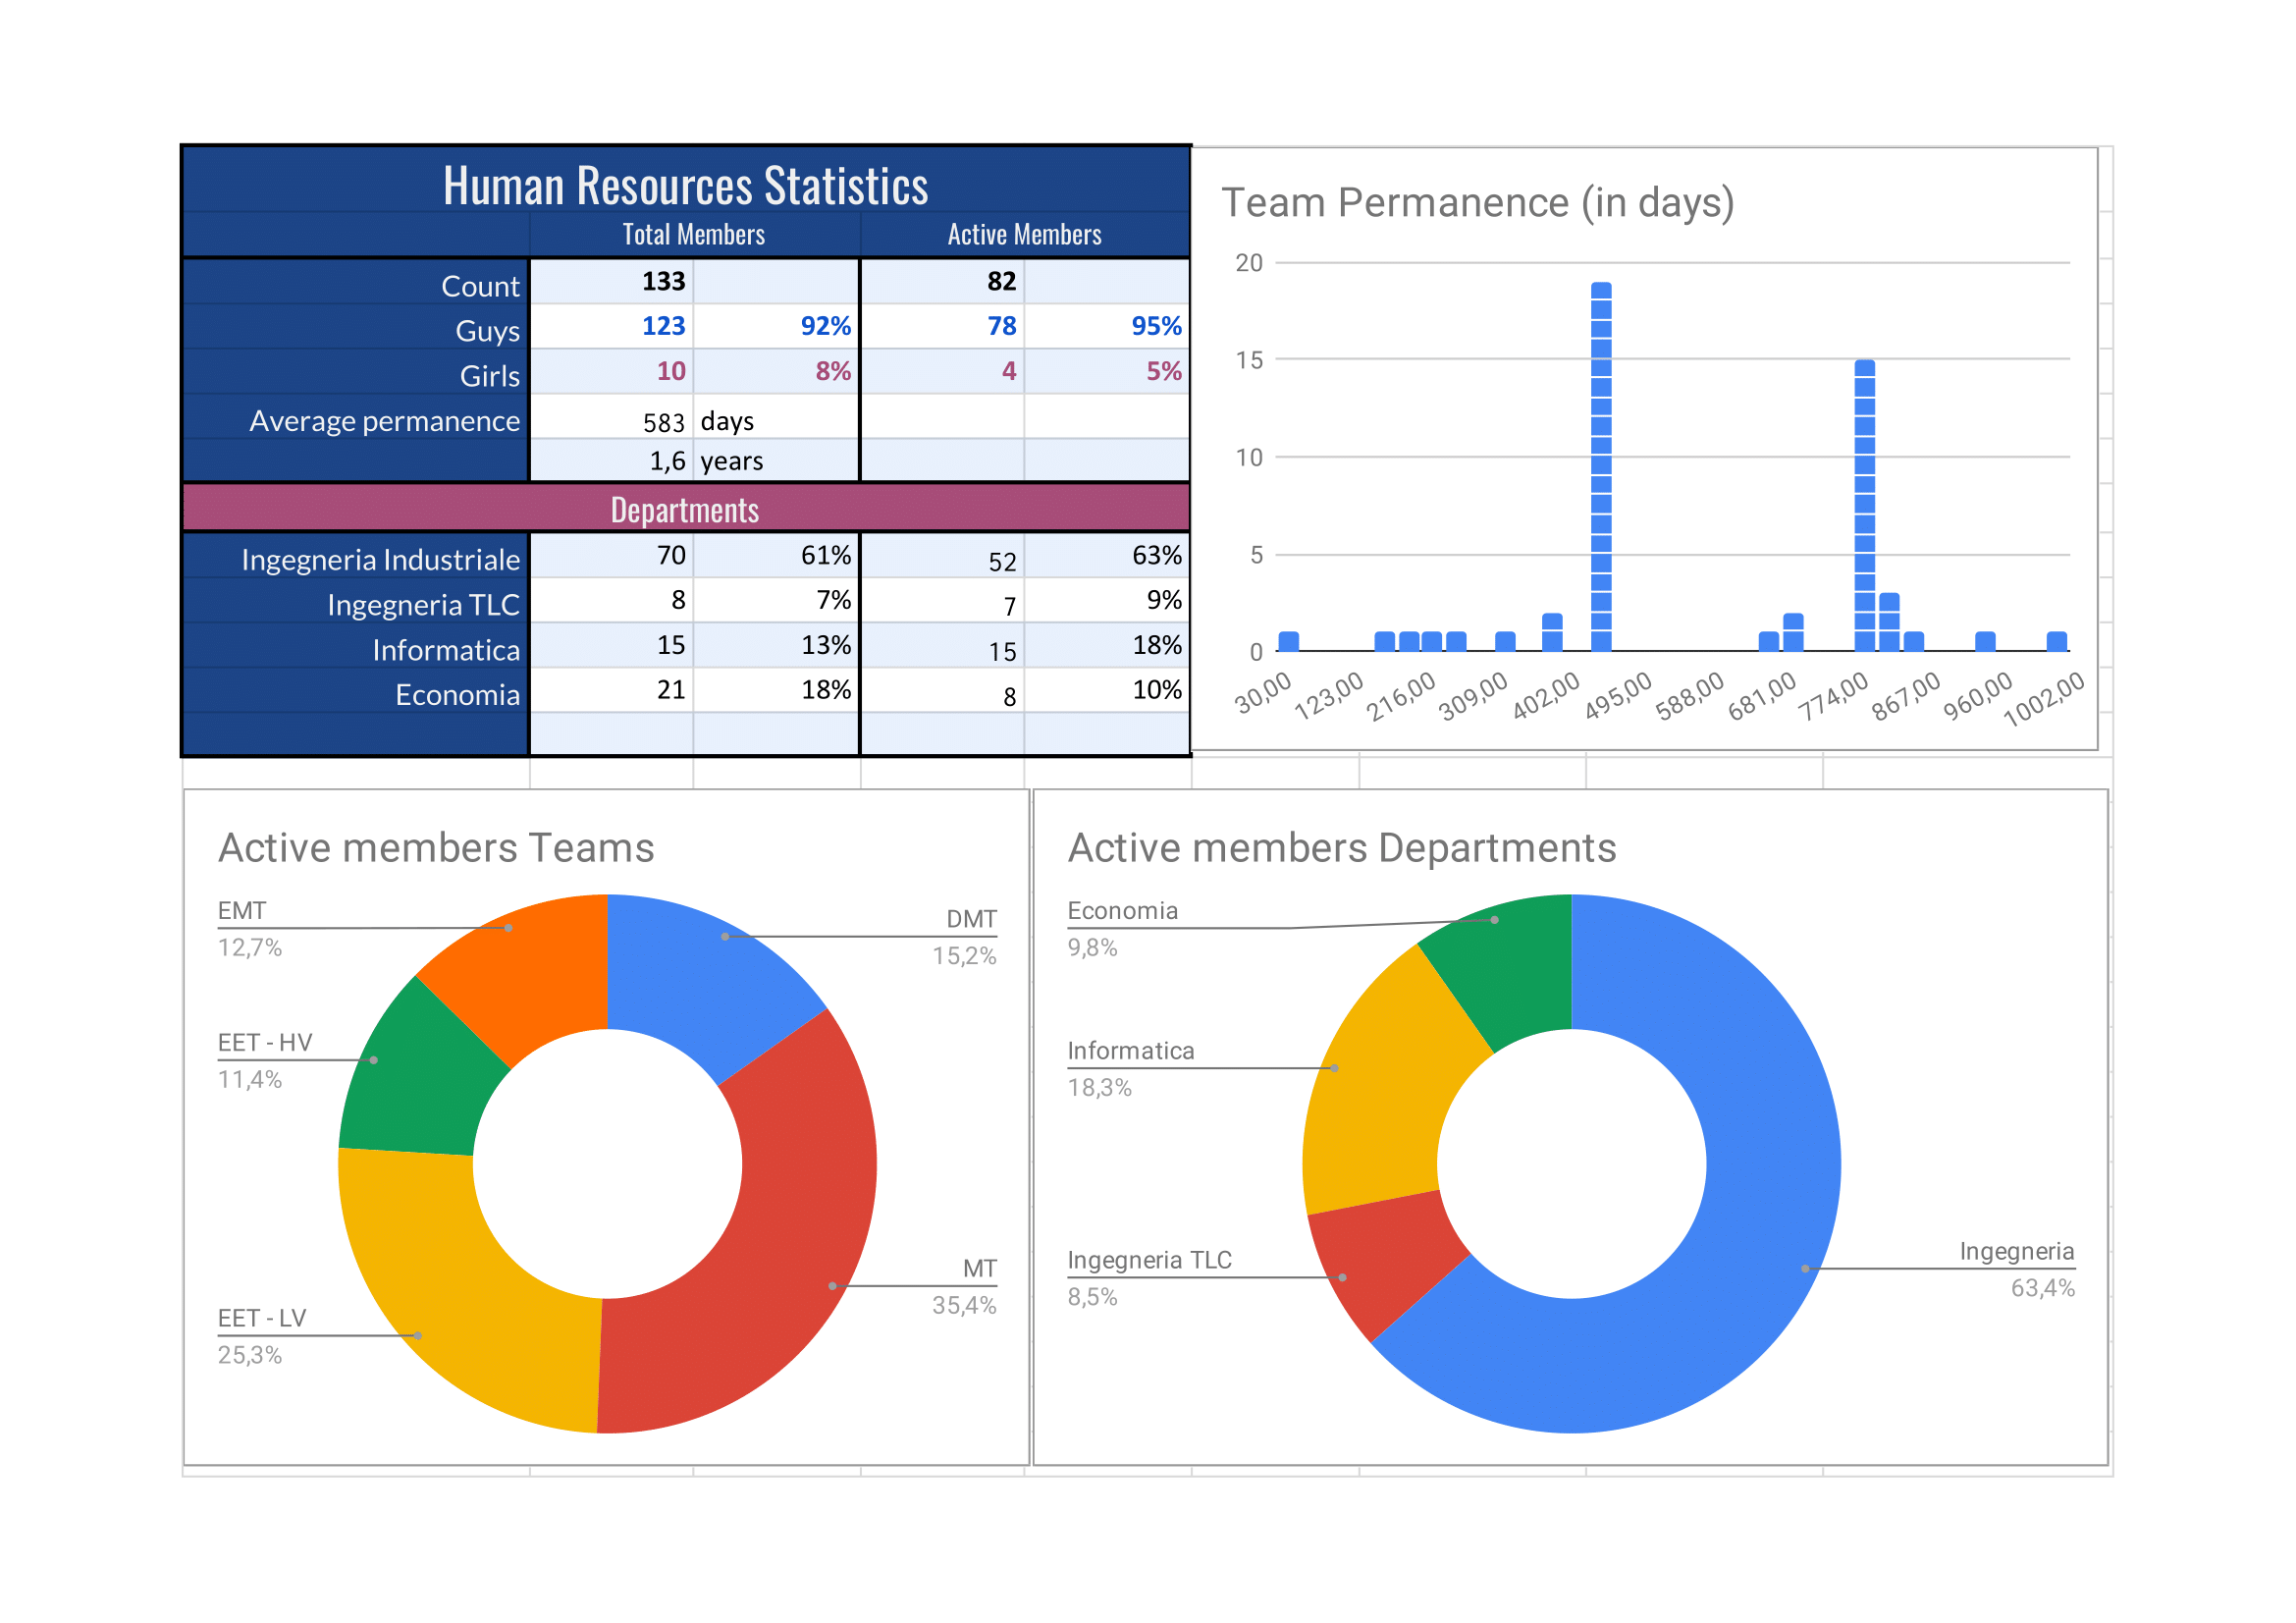
\includegraphics[width=0.75\textwidth]{./figures/membri.png}
  \caption{E-Agle Trento Racing Team}
\end{figure}

L'organizzazione del Team a Settembre 2017 dal punto di vista software non era ben definita, 
alcune parti di codice erano presenti online, altre solo mantenute in locale dalle persone interessate.
Questa modalità ha avuto molti limiti, soprattutto per quanto riguarda il version controlling e l'aggiornabilità del codice, 
non avendo la possibilità di mantenere diverse versioni in paralello.
Per cui confrontadoci con gli altri studenti si è deciso di avere un profilo pubblico della squadra su GitHub per poter mantenere il codice
secondo gli standard attuali e poterlo condividere con chi d'interesse. La scelta di GitHub è stata spontanea, dovuta ai suoi vantaggi rispetto
a BitBucket per la partnership con l'unversità e quindi tool inclusi.
Questo ha migliorato notevolmente il workflow di chi lavorava sulle varie parti della macchina e il tempo di apprendimento degli studenti che hanno deciso di avvicinarsi al progetto
soprattuto grazie alla realizzazione, attraverso Sphinx e GitHub Pages, di una raccolta di documentazioni e procedure da tramandare. 

\newpage

\section{GitHub e Documentazione}

I due principali strumenti introdotti sono stati GitHub per il version controlling e 
la condivisone del codice e Sphinx per generare documentazione partendo da documentazioni che altri studenti avevano già scritto.

L'approccio a GitHub è stato lento, ma ha permesso di poter dare uno spazio a tutto il codice del Team in breve tempo.
Le repository sono gestite da un admin che si occupa di aggiungere gli studenti interessati e consiglia come mantenere il codice grazie a controlli periodici.
La struttura delle repository è definita in base alla monoposto e al sottogruppo di interesse, o più in generale una parte della macchina. 
Un esempio sono le due versioni del Volante, \emph{chimera-steeringwheel} \cite{chimera-telemetria} e \emph{fenice-steeringwheel} \cite{fenice-steeringwheel}.
Per quanto riguarda la repository del Volante è stato deciso di mantenerla pubblica.
Essendo un progetto universitario che vede l'impegno di più persone sotto più ambienti (software, hardware e meccanico)
ci è sembrata la scelta giusta presentare l'esempio di una interfaccia unica nel suo genere che utilizza diverse tecnologie
da cui le persone possono ispirarsi e utilizzarla come esempio per le librerie del framework e le tecnologie usate.

L'introduzione di Sphinx è nata dalla necessità di condividere le conoscenze con altri studenti che si avvicinano al progetto 
e trovare un punto raccolta unico e accessibile da esterni del materiale ritenuto utile e non sensibile.
La scelta di utilizzare Sphinx come strumento è dovuta alla consultazione, in quel periodo, di alcune documentazioni relative a schede
programmabili con Python. Questa documentazione mi è sembrata fin da subito semplice e facilmente mantenibile da parte di tutti.
Una delle prime guide pubblicate è stata \emph{"Come cross-compilare per Raspberry da Linux"} per il framework Qt, 
siamo partiti da una guida trovata su Medium \cite{Medium} per arrivare alla nostra versione per il Team Telemetria.
La scelta di utilizzare Sphinx come generatore di documentazione ha mostrato un grande vantaggio quando è stato deciso di rendere pubblico 
il materiale della Design Presentation. 

\begin{figure}[!hbt]
  \centering
  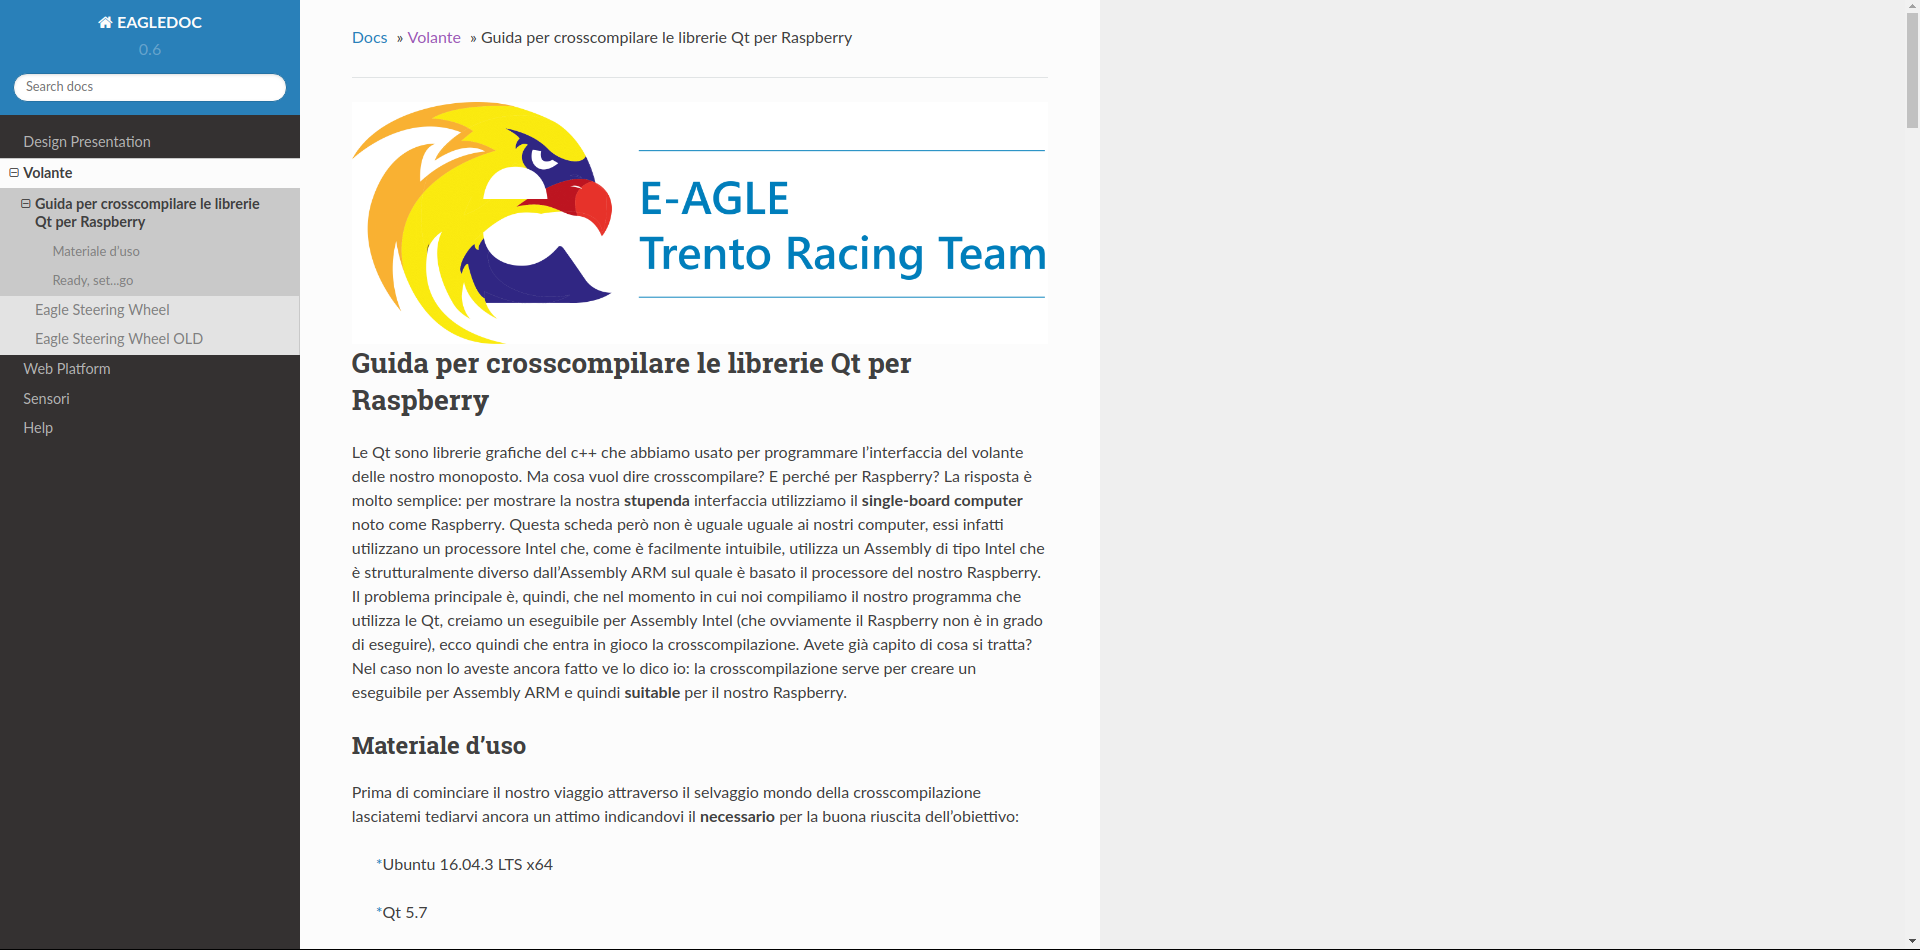
\includegraphics[width=0.75\textwidth]{./figures/sphinx.png}
  \caption{Sito Documentazione del Team \cite{eagletrt.github.io}}
\end{figure}

Questi materiali sono stati portati dal formato \emph{.docx} a \emph{.rst}, utilizzato da Python per creare pagine \emph{.html} statiche.
Sono state poi rese disponibili online e accessibili attraverso QR code dai nostri rollup che esponiamo durante gli eventi.
Il risultato è stato quello di poter mostrare agli sponsor e alle persone interessate al progetto il lavoro svolto per ogni componente realizzata da noi
e le scelte tecniche fatte.

\newpage

\section{Organizzazione Team e Attività}

% Sviluppo agile perchè ci è sembrata la più adatta
% Tavole Kanban per tutti grazie a waffle.io
% Divisione Team 

Durante le riunioni con il gruppo telemetria ho riscontrato delle difficoltà da parte dei membri
nell'organizzazione del lavoro e nell'avere chiari gli step necessari per il raggiungemento dell'obbiettivo principale.
Per ovviare a questo problema si è rivelato molto utile un approccio \emph{agile} e l'utilizzo di tavole \emph{kanban}.

Predisporre il team all'utilizzo di metodi agili ci ha permesso di ridurre il rischio di fallimento 
durante lo sviluppo, testando in locale e poi portando in macchina la funzionalità senza riscontrare errori.
Il problema principale che emerge dai partecipanti al progetto è quello di non poter dedicare
il tempo che desiderano al team, avere un approcio \emph{agile} ci ha permesso di sviluppare in breve tempo e in modo 
ordinato tutto quello che ci veniva richiesto venendo incontro alle esigenze dei singoli.

Il risultato è stato un approccio diviso in queste fasi:
 
\begin{itemize}
  \item Pianificazione: Determinare, concordando con i membri del team attraverso riunioni e/o resoconti dei test, quale funzionalità deve essere implementata.
  \item Analisi dei requisiti: Come può essere integrata la funzionalità all'interno del nostro codice, valutando librerie e tecniche alternative.  
  \item Progettazione: Divisa in due parti, la prima, molto importante nel nostro caso, disegno su carta per poi passare alla seconda che riguarda la stesura del codice. 
  \item Test: Svolti principalmente in locale e poi portati sul dispositvo senza riscontrare problemi di compatibilità.
\end{itemize}

Per quanto riguarda il Volante inteso come \emph{"prodotto finito"} i passi necessari sono stati più articolati.
Tutti i membri del gruppo si sono occupati di raccogliere delle possibili soluzioni per poi essere discusse e
confrontate anche con chi non era coinvolto direttamente, per poter condvidere il più possibile il \emph{know-how}.
Attraverso riunioni periodiche e la raccolta di feedback sulla nostra monoposto è stato possile, grazie alla disponibilità
delle persone coinvolte, di avere sempre chiaro cosa andava e cosa no. 
Questo è stato molto importante perchè ha definito una tipologia di task specifica che ogni membro del team, non per forza 
coinvolto nello sviluppo software, doveva portare a termine.

\begin{figure}[!hbt]
  \centering
  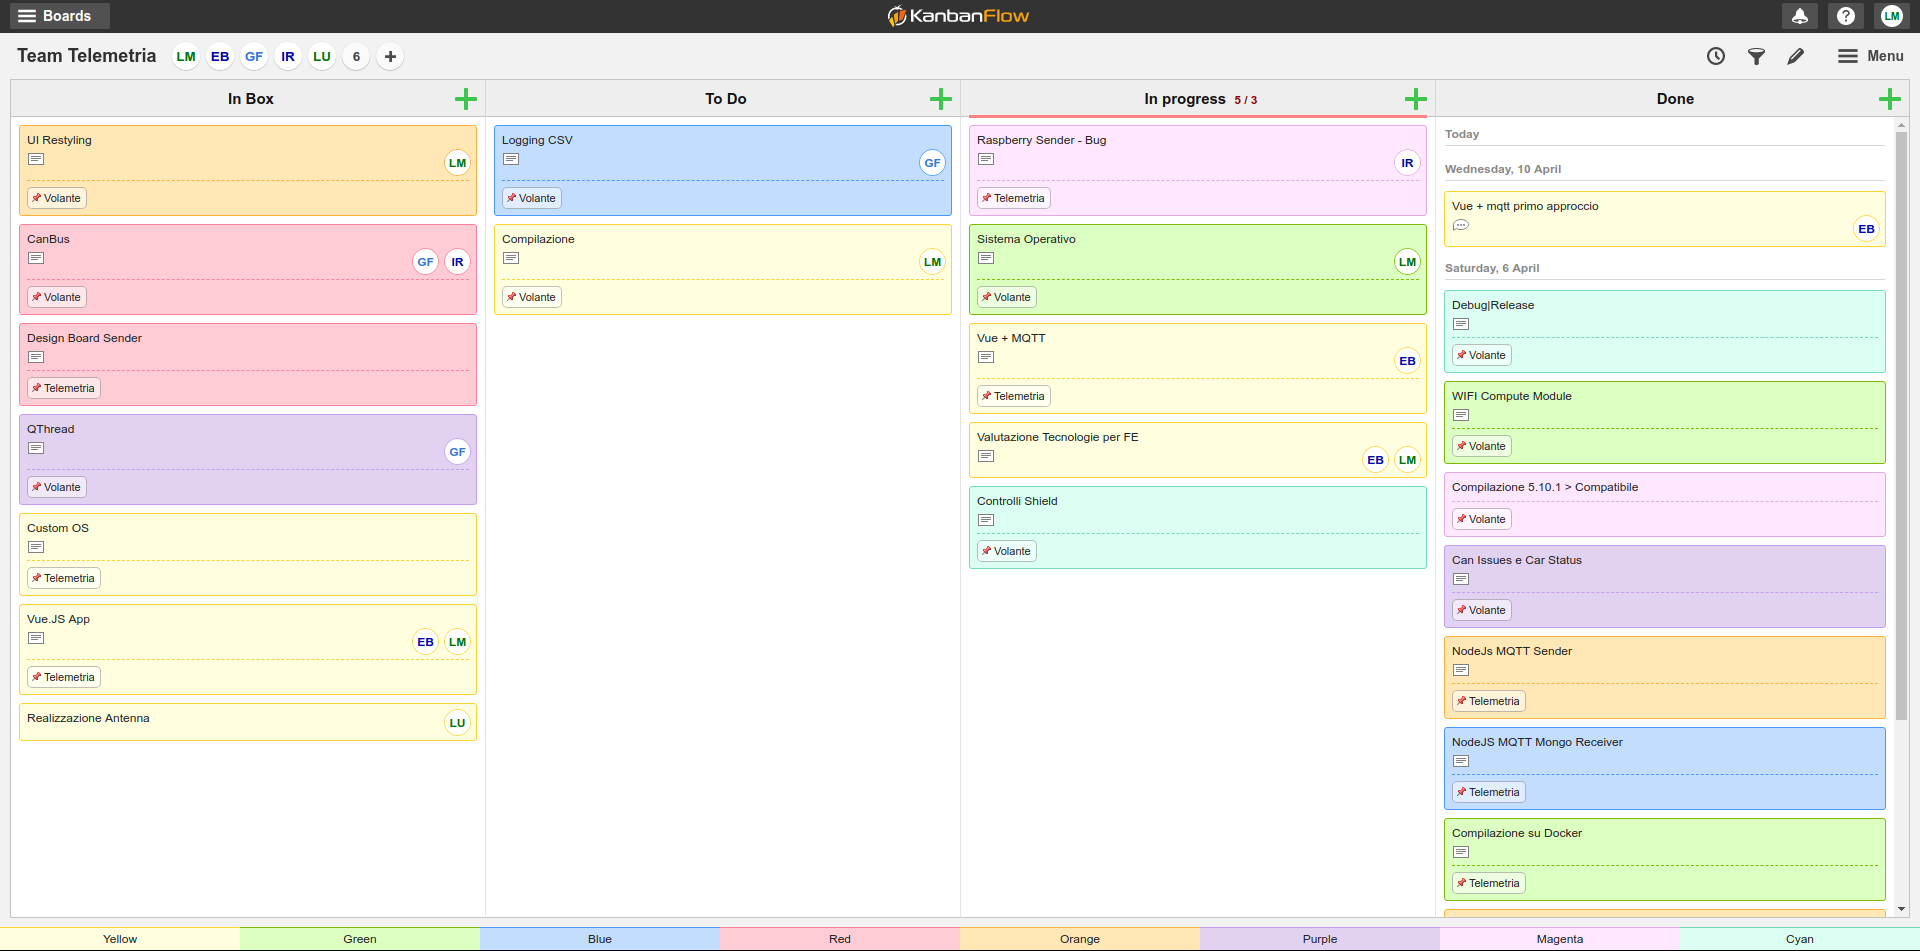
\includegraphics[width=0.75\textwidth]{./figures/kanban.png}
  \caption{Tavola Kanban utilizzata dal Team Telemetria}
\end{figure}

L'introduzione di Kanban ha migliorato il flusso di lavoro, aumentato la produttività e la qualità del prodotto finale in modo considerevole. 
Kanban fa parte dei metodi agili e come tale rende il processo lavorativo molto più flessibile, 
non sempre le task sono state portate a termine nelle scadenze prestabilite, 
questo per impegni universitari e mancanza di esperienza nello stimare i tempi. 
I compiti sono stati suddivisi in piccole task e portati a termine l’uno dopo l’altro. 
Tuttavia data la sua flessibilità abbiamo sempre mantenuto indipendete lo sviluppo di una parte rispetto ad un'altra e grazie alla facilità 
di creare prototipi in grado di testare le singole funzionalità in poco tempo non si sono mai trovate delle situazioni in cui non potevamo testare 
perchè non avevamo un finito una task. 
Lo sviluppo in parallelo, considerato come attività multitasking, è stato sempre mantenuto in quanto le competenze dei singoli membri del team erano sempre 
abbastanza specifiche. 

Il team che si è occupato dello sviluppo del Volante e della sua realizzazione è composto da:
\begin{itemize}
  \item Davide Farina: Pilota e supervisore del progetto
  \item Luca Martinelli: Main Developer
  \item Daniele Faccinelli: PCB Designer 
  \item Laura Scoccianti: UI Designer
  \item Ciro Malacarne: Case Designer
  \item Damiano Iob: Responsabile del Sistema Operativo
\end{itemize}

Ogni parte dello sviluppo è stata messa su Gantt e poi, per avere una visione specifica del lavoro, 
le fasi del Gantt sono state espanse e analizzate come tante singole task identifiacando poi la fine come una \emph{Milestone}.
Nel 2019 come strumento è stato utilizzato \emph{waffle.io}, in quanto è facilmente integrabile con la repository GitHub.
Quest'anno, invece, causa la chiusura del sito, ci siamo spostati a \emph{Kanban Flow} perchè non avendo esigenze particolari qualsiasi applicazione web
poteva fare al caso nostro. L'unico requisito è stato la semplicità d'uso e avere più progetti nello stesso tempo.
Gli studenti coinvolti, anche se non direttamente interessati allo sviluppo software, utilizzavano la tavola kanban per avere sempre sotto 
mano lo stato dei lavori. Per quanto riguarda la creazione di nuove task, e più in generale, la sua gestione, se ne è occupato l'amministratore. 

% conseguenze? scelte tecniche (e) specifiche vincenti grazie al confronto di persone diverse con lo stesso scopo

Una considerazione importante da fare è che questi problemi sono emersi durante la mia presenza nel team e precedentemente non erano mai stati rilevati.
Lo scopo principale fin da subito è stato la realizzazione della macchina e mentre c'è stata attenzione per l'organizzazione in senso 
generale si è trascurato l'aspetto organizzativo del singolo sotto-team e in particolare dello sviluppo software. 
Le motivazioni sono da trovare nel breve tempo che si ha a disposizone per sviluppare e testare e nell'inesperienza delle persone coinvolte
visto che il progetto è nato da poco e dobbiamo confrontarci con studenti di facoltà 
che hanno squadre con esperienza di oltre 10 anni di competizione.  
L'introduzione di queste tecnologie e la formazione delle persone per approcciarsi ad ess,e ha fatto si che le scelte tecniche potessero essere
prese con più consapevolezza, alle volte in modo indipedente, grazie alla divisione dei compiti in base alle aree di competenza. 
Scelte che si sono poi rivelate vincenti nel corso del progetto.

\newpage

% Durante la sessione invernale, quando decisi che avremmo dovuto ridisegnare l'interfaccia, stavo seguendo il corso di ingegneria del software 2 e sostenendo l'esame di ingegneria del software 1, questo mi ha permesso di mettere in pratica le nozioni teoriche apprese a lezione.
% Questa è stata un parte molto importnate per lo sviluppo di un progetto così vasto in termini di conoscenze di settori specifici, avere chiaro fin da subito il ruolo di ognuno nel team è stato di grande aiuto. 
% Oltre ad averci permesso di ridurre di molto i tempi di sviluppo e test, ci ha dato la possibilità di essere apprezzati da specilisti nel settore non solo per il prodotto ma anche per come sono state affrontate e prese le scelte.

% Il nostro obbiettivo è stato sin da subito fare qualcosa di unico e che altre squadre e case automobilistiche avrebbero potuto vedere, da qui l'esigenza di rendere il codice pubblico  

    \chapter{Tecnologie}

\begin{figure}[hbt!]
    \centering
    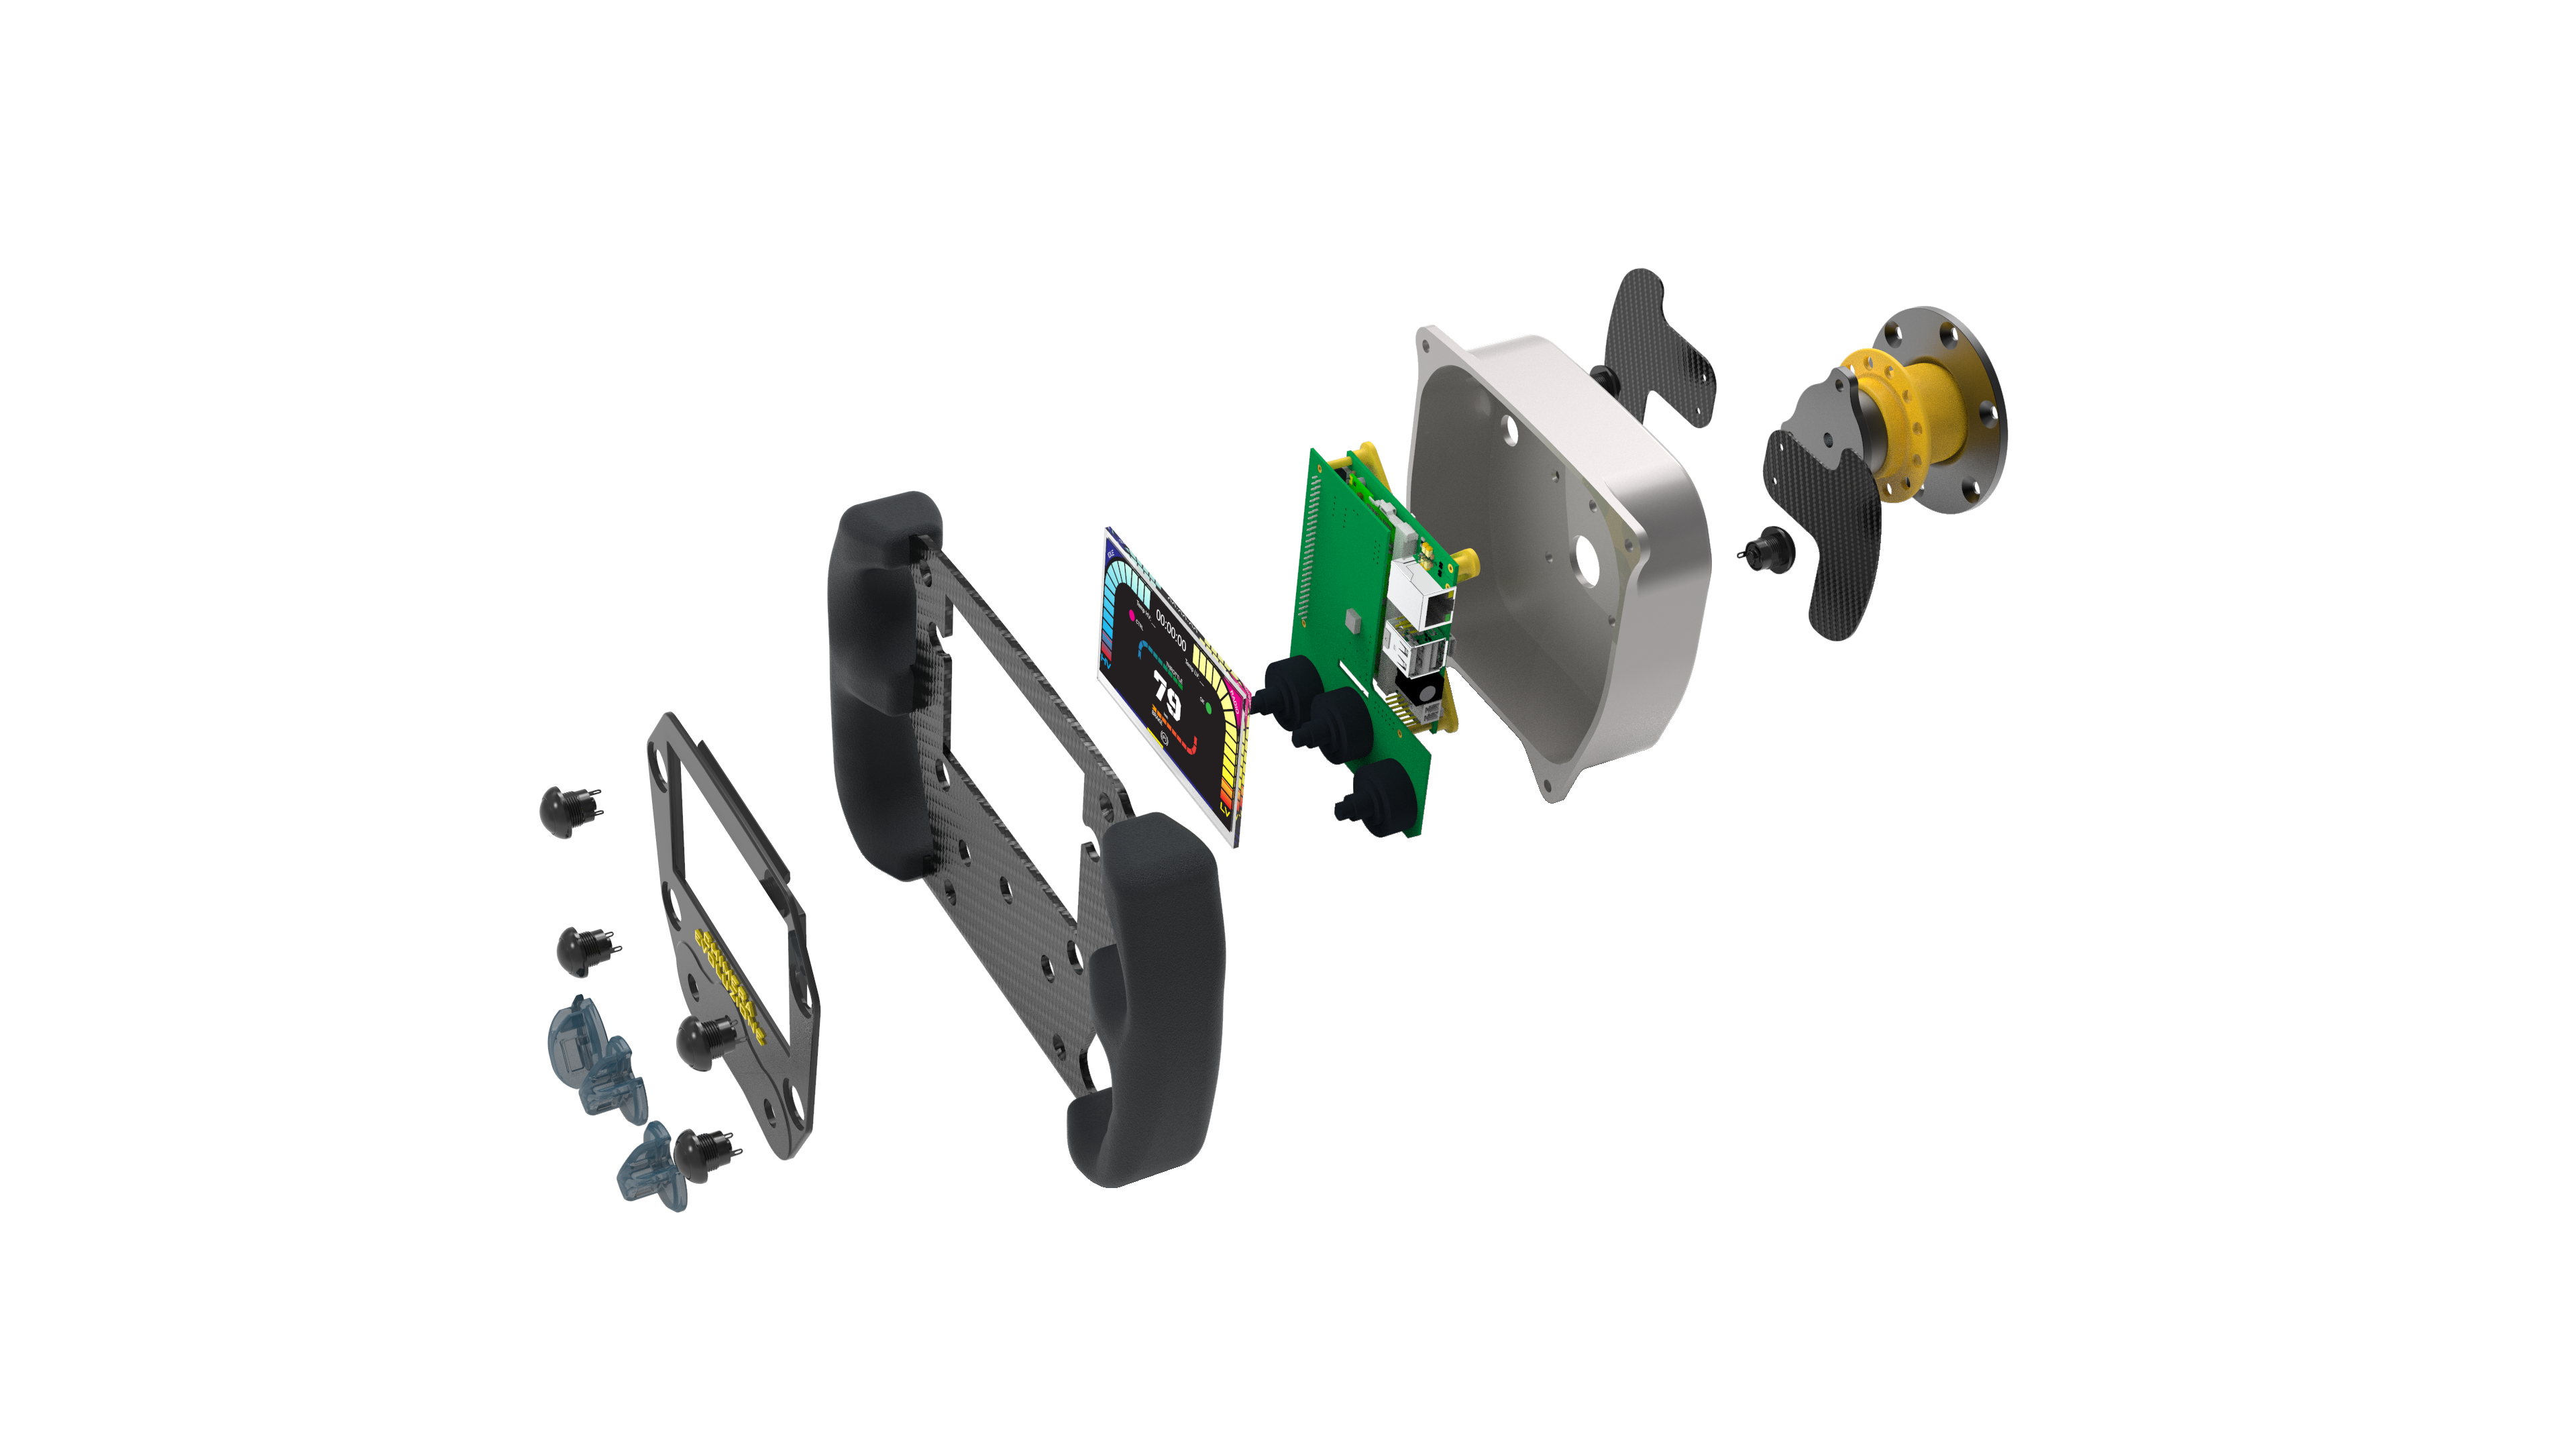
\includegraphics[width=1\textwidth]{./figures/steeringwheelEsploso.png}
    \caption{Esploso del Volante}
\end{figure}

% grazie al confronto di studenti e professori -> idee vincenti 
Durante l'intero progetto del Volante si è sempre cercato di confrontarsi con professori competenti nel settore di referimento.
Questo ha portato ad acquisire sempre più idee possibili per poter trovare soluzioni ottimali e innovative ai nostri problemi.
L'interdisciplinità del progetto ha fatto si che professori, provenienti anche da dipartimenti diversi avessero la possibilità di dare importanti 
contributi e utili consigli, su quali tecnologie potessero fare al caso nostro.
Questo ha fatto si che ogni singola scelta dovesse essere motivata e costruita da una base di esperienze personali facoltative e considerazioni
giustificate con esempi. Queste scelte sono poi state discusse in gruppo per essere approvate da tutti.
Le scelte prese sono state abbastanza indipendenti, considerando il settore meccanico e software/elettronico, considerando le limitazioni che si potrebbero affrontare.
Non si sono verificate situazioni in cui una nostra possibile scelta non potesse essere presa vedendo come ostacolo ad esempio il case del Volante.
Le difficoltà invece si sono ritrovate nel interfacciare il sistema operativo con l'hardware che, per nostra inesperienza, ha portato ad alcune 
situazioni in cui i lavori sono rallentati.   


\newpage


\section{Scelta del Hardware}

\begin{figure}[hbt!]
    \centering
    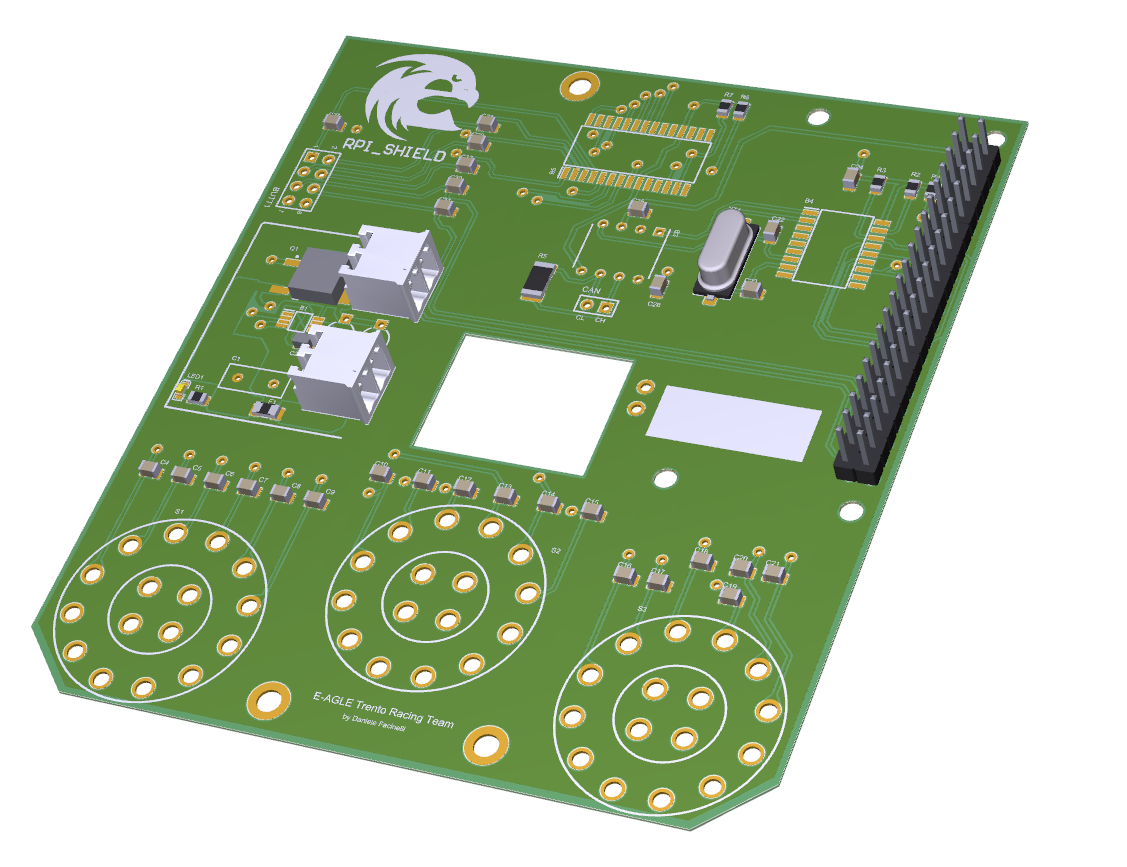
\includegraphics[width=0.75\textwidth]{./figures/imageshield.png}
    \caption{Shield del Volante}
\end{figure}

%   perchè abbiamo scelto raspberry pi zero (linux), 
%   in cosa ci ha avvantaggiato (money) (facilità di averla) (sostituirla con altre schede)
%   Funzionamento Shield

La scelta della scheda si è basata principalmente su due aspetti molto importanti, il prezzo e la facilità di sviluppo.
Dopo aver fatto ricerche per la compatibilità di diversi software l'utilizzo di un Raspberry è risultato sin da subito la scelta 
più pertinente dato il nostro backgorund di studenti appassionati di elettronica e software.
In particolare la nostra attenzione è caduta su Rasberry Pi Zero un dispositivo low cost, con la possibilità di avere una connessione 
wifi on-board (facilità di collegarsi ad AP), dimensioni e peso ridotte e adattabile a diversi dispositvi di input/output.
Raspberry vanta una community di appassionati e sviluppatori nel settore informatico molto vasta, questo ha permesso di trovare 
esempi e documentazione con facilità.
Raspberry Pi Zero può essere poi aggiornato alle versione più performanti senza troppi problemi, montando un processore ARM 
prodotto dalla casa Broadcoam, nel nostro caso (BCM2835), necessità solo di aggiustamenti software, mantenendo uguale l'ambiente software.
Ciò che rende unico il nostro Volante è il fatto di essere custom in tutte le sue parti.
Per necessità è stata disegnata una shield collegata ai GPIO del Raspberry 
per poter aumentare e utilizzare al meglio le sue funzioni di input e output.
Per quanto riguarda le interfacce di input del pilota, per poter utilizzare più tasti e più manettini (3 manettini da 6 posizioni), 
è stato introdotto sulla shield un I2C multiplexer, precedentemente utilizzando un solo manettino non era necessario.
Come display è stato scelto di utilizzare un LCD 4.3" TFT, collegato alla scheda via HDMI, grazie a un modulo di \emph{Adafruit} per poter
avere una maggiore scelta, in quanto sul mercato momentaneamente per quanto riguarda le  specifiche tecniche i display che 
escono direttamente in HDMI hanno una luminosità troppo bassa per poter essere usati sotto il sole. 
Le nostre necessità sono state, dal punto di vista del pilota, di avere quattro tasti fisici nella parte frontale 
per poter utilizzare l'interfaccia, due paddle per potersi muovere nelle diverse tab e 
tre manettini per poter gestire la configurazione della macchina.
Per quanto riguarda invece l'interfaccia di comunicazione con il resto della macchina si è reso necessario l'utilizzo del SPI
per poter comunicare in Can-Bus utilizzando l'MCP2515 e l'alimentazione, che passa per il sistema di aggancio rapido, per poter alimentare il Volante a 5V.



\newpage


\section{Scelta del Case}

\begin{figure}[hbt!]
    \centering
    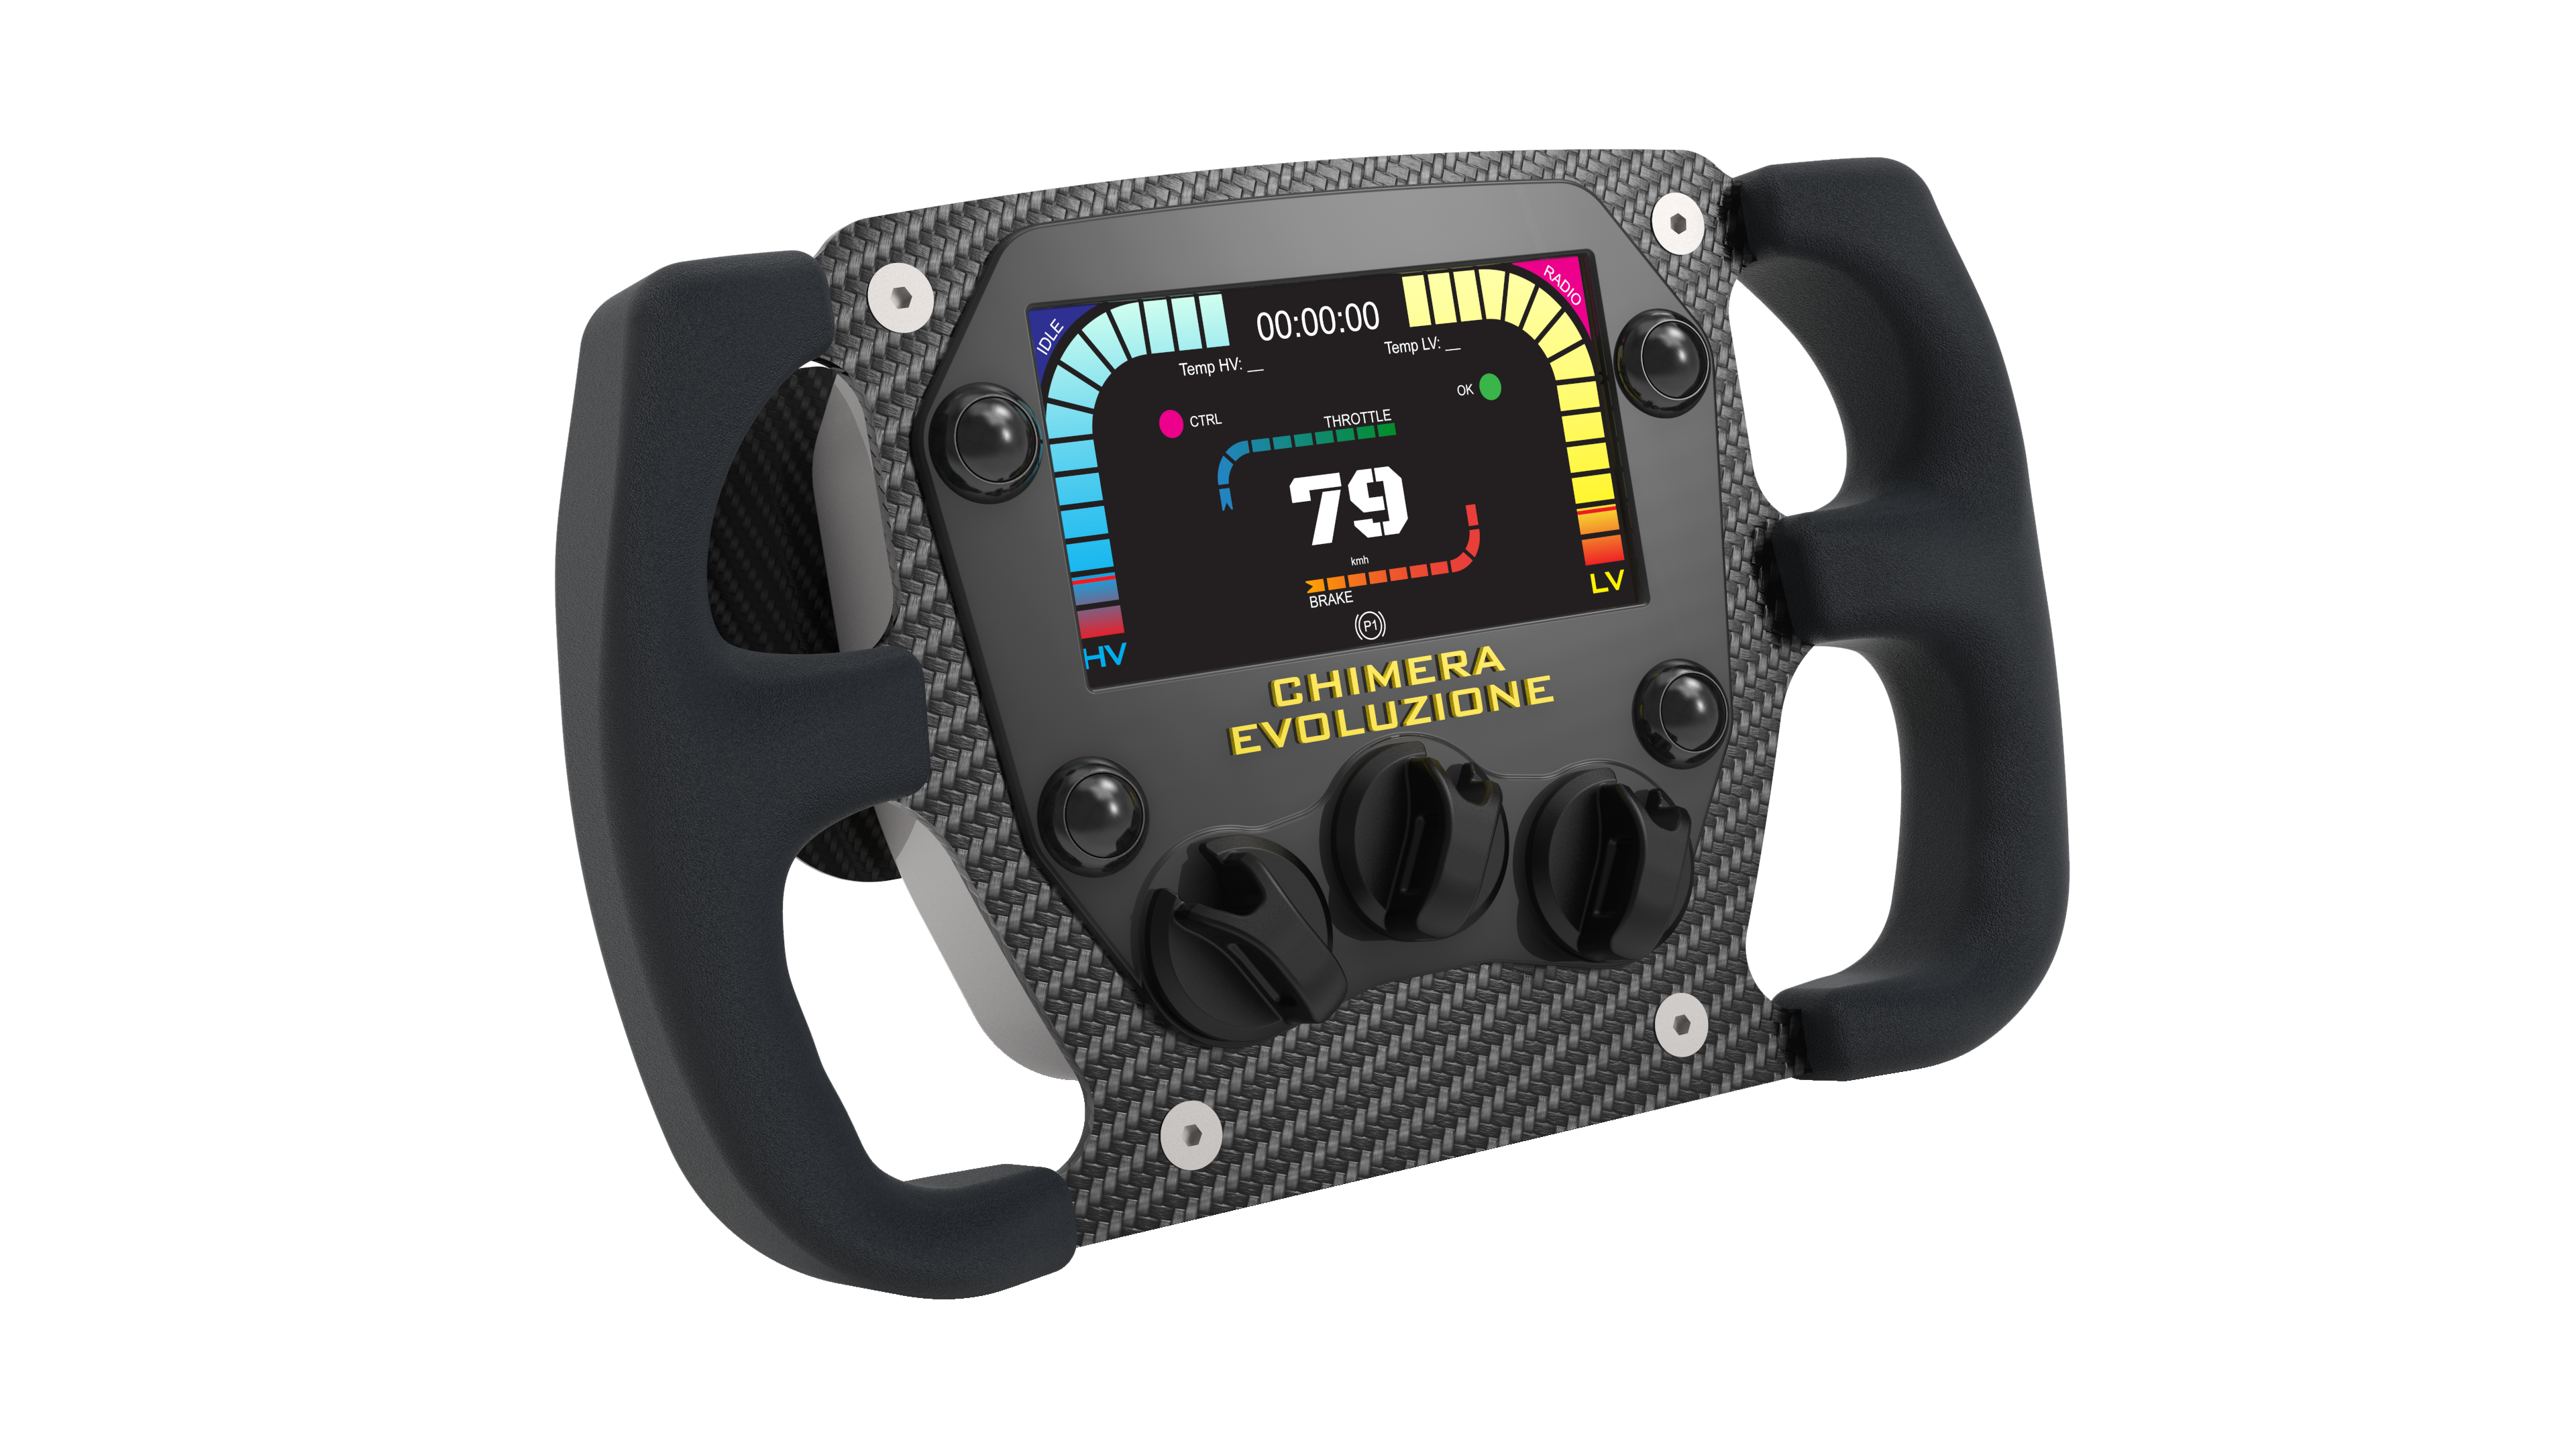
\includegraphics[width=1\textwidth]{./figures/imagemockup.png}
    \caption{Primo Mockup del Volante di Chimera Evoluzione}
\end{figure}

% Parte tradotta di Ciro e con giustificazioni sulla forma date dalla dimensione della scheda interna, costruitto attorno

La scelta di ridisegnare il case, rispetto al modello del'anno precedente 
nasce dall'esigenza di avere una maggiore ergonomia, una maggiore usabilità
e la possibilità di aggiornare le funzionalità in corso di sviluppo.
I materiali utilizzati nella versione precedente non erano adatti 
ad un uso sotto stress e non risultava facile il debug della componentistica hardware
in fase test. 
Per quanto riguarda il design del Volante di Chimera Evoluzione le scelte 
sono state prese per soddisfare il regolamento e valutando lo spazio all'interno
riservato alla componentistica elettronica.
I requisti che abbiamo considerato sono stati una maggiore robustezza, ergonomia
qualità dei materiali, facilità di assemblaggio ed estetica per venire incontro 
alle esigenze del pilota.
Per la parte di produzione è stata fatta una ricerca sulle migliori soluzioni che potevamo
utilizzare per costruirlo e con i materiali che più venivano incontro alle nostre esigenze.

Tutte le componenti sono state disegnate e realizzate dal team nei nostri laboratori.

\begin{itemize}
    \item Piastra Principale: fibra di carbonio con core interno in schiuma da 1.5 mm per uno spessore totale di 3 mm, trattamento di cura in autoclave. Rifinito con tecnologia di taglio ad acqua per ottenere la forma desiderata.
    \item Paddle: 5 strati di fibra di carbonio, Trattamento di cura in autoclave, rifinito con taglio ad acqua.
    \item Mascherina Frontale: Stampata in 3D con processo di stereolitografia, Materiale: Resina, Stampante: Form 2
    \item Manettini: MJF (Multi Jet Fusion) with HP Jet Fusion 3D 4200 printer, PA 12 powder, sandblasted and painted
    \item Imppugnatura: Stampata in 3D con processo di stereolitografia, Materiale: Resina, Stampante: Form 2. Incollati con adesivo strutturale.
    \item Guscio Posteriore: Alluminio serie aeronautica, lavorato da un blocco grezzo con fresa CNC a 5 assi
\end{itemize}


\newpage


\section{Scelta del Sistema Operativo}

\begin{figure}[h!]
    \centering
    \begin{minipage}{0.5\textwidth}
        \centering
        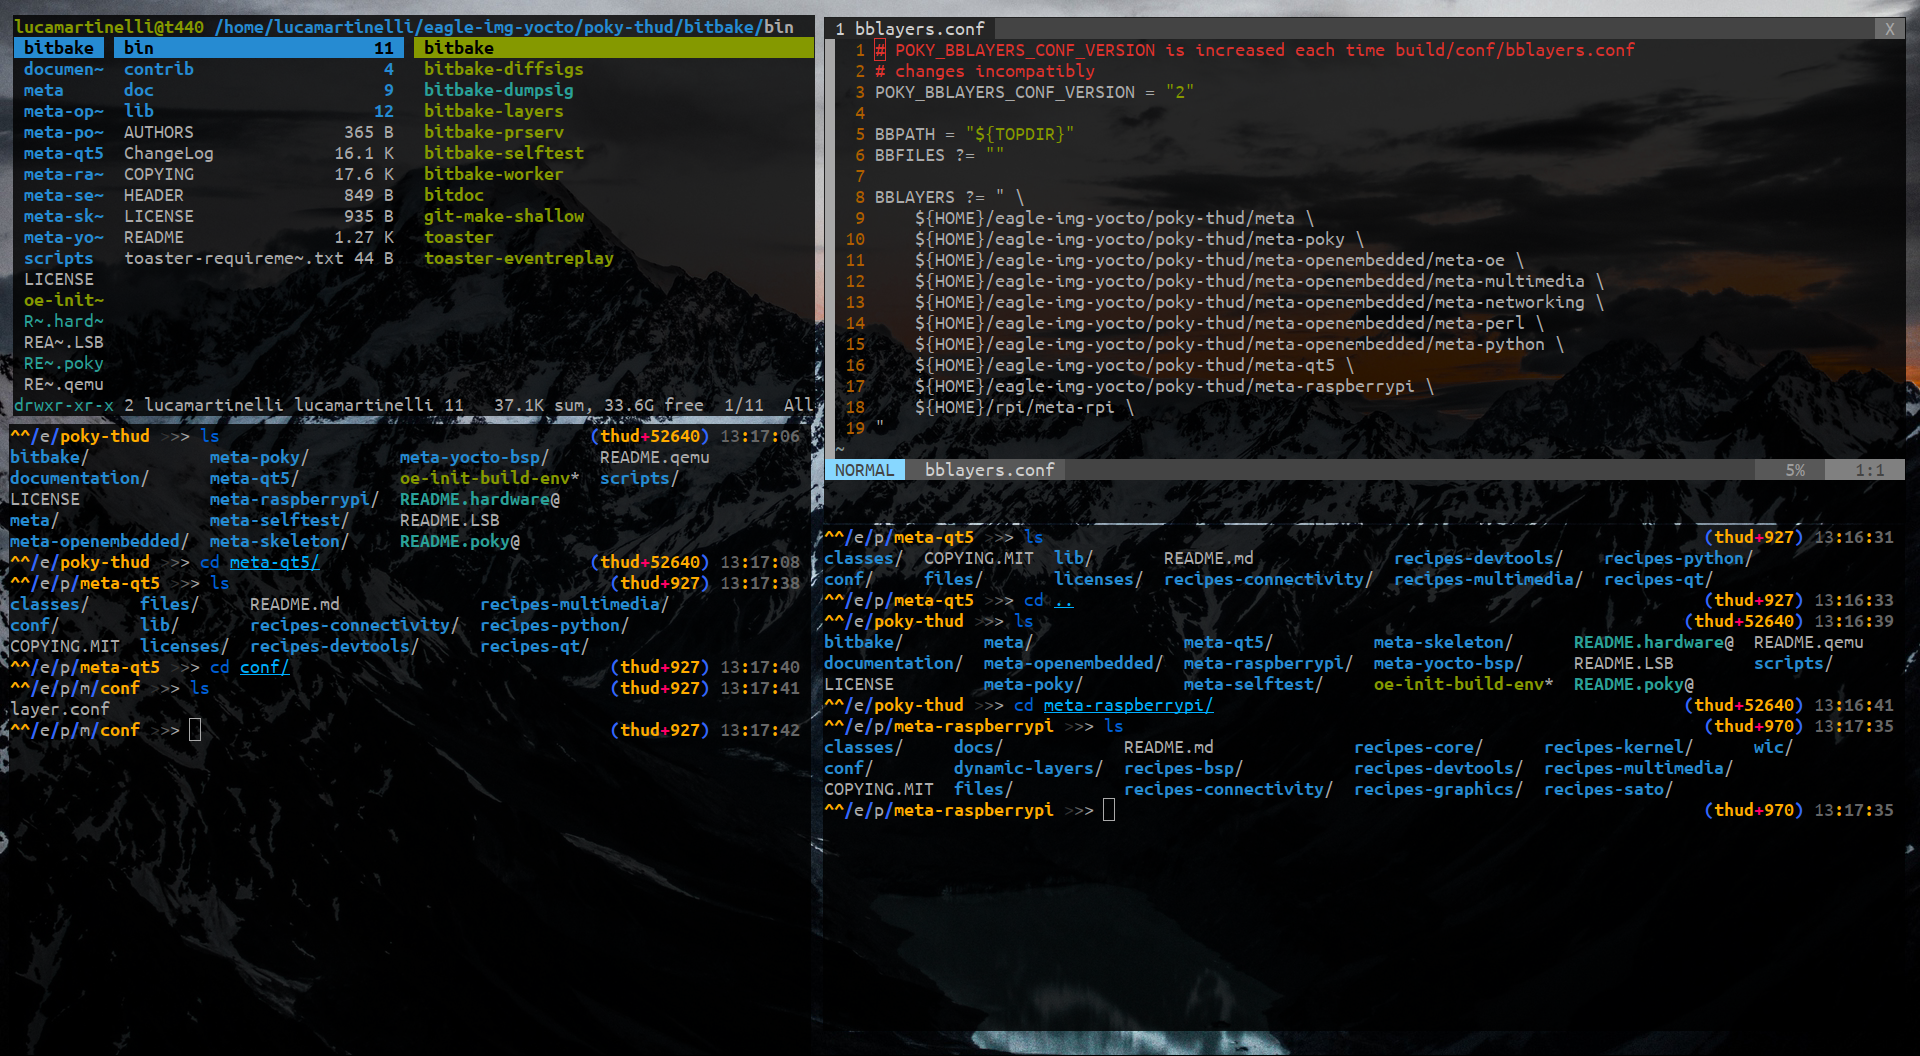
\includegraphics[width=8cm]{./figures/yoctoWorkFlow.png} % first figure itself
        \caption{Yocto preparazione dell'ambiente}    
    \end{minipage}\hfill
    \begin{minipage}{0.5\textwidth}
        \centering
        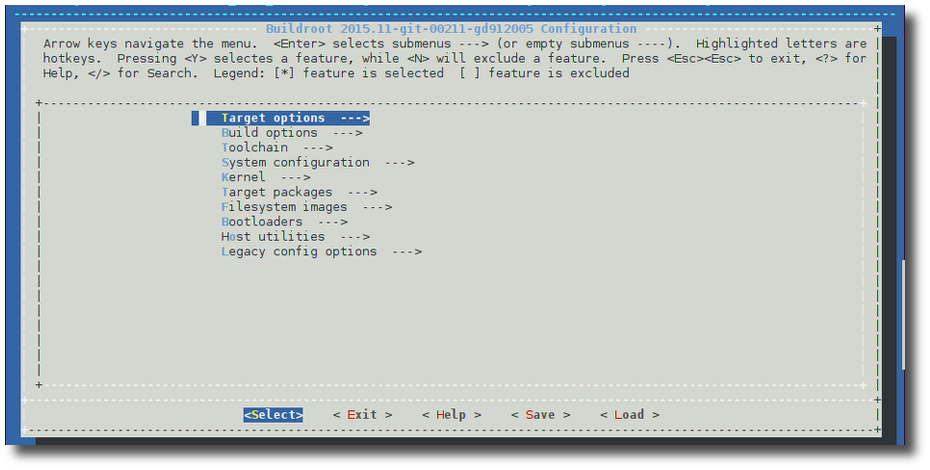
\includegraphics[width=8cm]{./figures/menuBuildRoot.png} % second figure itself
        \caption{Builroot - Primi passi della fase di build}        
    \end{minipage}
\end{figure}

% debug di linux e facilità di implementare funzionalità in breve tempo 

La scelta della scheda ci ha portato ad utilizzare in fase di test una delle ultime
versioni stretch di Raspbian presenti nel 2017. Le ottimizzazioni sono state in termini
di boot time, l'autostart della applicazione, la connesione a reti wireless,
la configurazione dell'uscita hdmi per il display e le librerie necessarie per poter eseguire il programma. 
I nostri requisiti sono stati principalmente due, il poter compilare senza dover utilizzare il Volante,
lasciando così il dispositivo il più leggero possibile e poterlo utilizzare come sistema di debug della macchina.
L'utilizzo di \emph{SocketCan}, attraverso il paccheto \emph{can-utils} ci ha permesso in più situazioni di gestire e leggere i messaggi
senza eseguire il software del Volante, ma come una macchina linux collegata ad essa via \emph{ssh} e per aggiornare il codice via \emph{scp}.
Una volta definiti tutti i requisiti e attraverso il progetto open-source \emph{buildroot} abbiamo sviluppato
un sistema operativo con tutte le specifiche richieste, successivamente le condizioni sono cambiate e
abbiamo deciso di spostarci verso un altro ambiente di cui è presente più documentazione che spiegherò nel prossimo sottocapitolo. 
Grazie alla diversificazione delle ricette è possibile aggiornare la componentistica hardware cambiando alcuni parametri 
prima della fase di build, questo ci ha permesso di mantenere una buona stabilità nel workflow senza dover mantenere più progetti, ma 
solamente di modificare la ricetta di quello già esistente e integrare i pacchetti necessari per la scheda di riferimento.
Mantenere lo stack di un sistema operativo Linux ha permesso di integrare facilemente le funzionalità dalla versione
desktop a quella in macchina, soprattutto per la cross-compilazione.
Durante il secondo semestre del 2018 per necessità del team mi è stato chiesto di verificare alcune soluzioni per poter avere un sistema operativo
\emph{"real-time"}, tra le possibilità la più interessante sulla quale ho fatto alcuni test e ricerche è risultata essere \emph{Xenomai}, ma per 
mancanza di tempo e sviluppatori il progetto è stato abbandonanto dovendo concludere lo sviluppo del Volante per Chimera Evoluzione.
Successivamente, grazie ai risultati ottenuti con il Volante, questo non è risultato più un problema avendo altre alternative più facili da implementare.

\newpage

\section{Scelta del Framework}

\begin{figure}[h!]
    \centering
    \begin{minipage}{0.5\textwidth}
        \centering
        
\includegraphics[width=8cm]{./figures/qtIcon.jpg} % first figure itself
    \end{minipage}\hfill
    \begin{minipage}{0.5\textwidth}
        \centering
        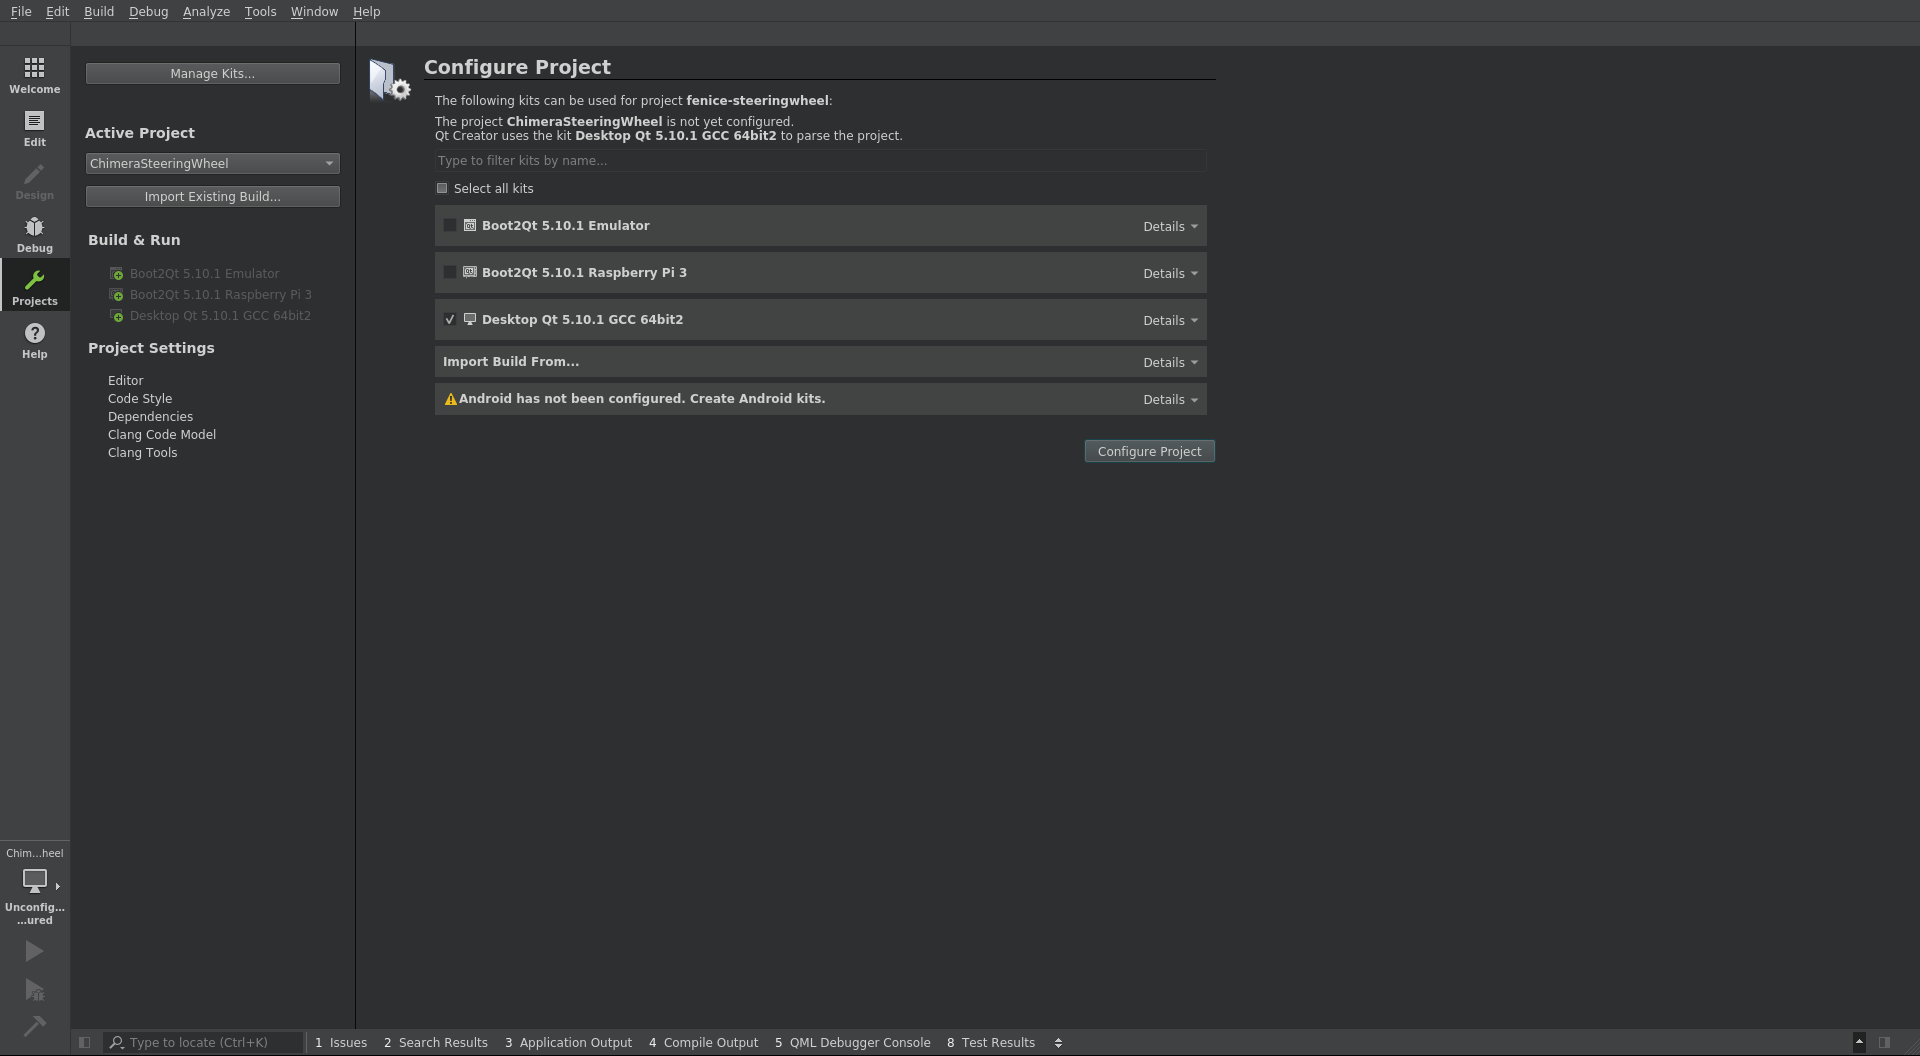
\includegraphics[width=8cm]{./figures/qtCreator.png} % second figure itself
        \caption{Qt Creator - apertura di un progetto e scelta del compilatore}                
    \end{minipage}
\end{figure}

%   perchè abbiamo scelto qt (buona base di partenza) e comodità di questo framework (compatibilità, multipiattaforma)
%   Discorso di sponsorizzazione e di conseguenza facilità di utilizzare i loro pacchetti con yocto

La scelta del framework era già stata fatta precedentemente il mio arrivo nel team, la decisione 
che è stata presa per Chimera Evoluzione è stata quella di voler terminare il lavoro dell'anno precedente 
aggiornarlo e renderlo il più possibile stabile e adatto alle nostre esigenze.
Il framework in considerazione risulta essere Qt, che permette grazie alle sue librerie grafiche 
multipiattaforma di lavorare in C++ e disegnare in breve tempo interfacce grafiche.
Qt, oltre ad essere utilizzato per soluzioni embedded, vanta numerosi esempi nel campo dell'automotive, è infatti 
presente nelle dash digitali di alcuni modelli nel mercato automobilistico.
I vantaggi di questo framework sono la diversificazione del lavoro in termini di sviluppo, chi si occupa 
di aggiornare la parte grafica, quindi il FE, non per forza deve essere in stretta relazione con chi sviluppa la parte
di backend del progetto, garantendo un workflow più dinamico. 
Qt nasce come framework open-source, i progetti che abbiamo preso in mano per capirne le potenzialità erano
sviluppati su Raspberry o comunque sistemi Linux e facilmente portabili a piattaforme embedded, non tanto per 
la parte di compilazione ma del progetto in senso stretto.
Inoltre Qt risulta abbastanza intuitivo al primo approccio utilizzando la sintassi di C++ ma, le prime difficoltà 
si riscontrano nell'utilizzare le funzioni proprietarie che, anche se fornite con una buona documentazione, non sempre
risulta completa.

Questo framework presenta anche una versione commerciale distribuita da \emph{The Qt Company}, 
con la possibilità di utilizzare \emph{tool} proprietari disegnati per facilitare il lavoro degli sviluppatori e ampliarne le funzionalità  
attraverso ulteriori librerie e pacchetti per compilare su dispositivi embedded.
Oltre alla community, che presenta sempre discussioni interessanti sulle nuove funzionalità implementate, con la versione commerciale
si ha a disposizione un servizio di assistenza e consulenza.    

L'accesso ai GPIO è stato gestito utilizzando le librerie di \emph{wiringpi} \cite{wiringPI} che, oltre a permetterci di gestire i singoli bottoni,
ci ha permesso grazie al multiplexer di leggere lo stato dei diversi encoder utilizzati come manettini. 

Nel Settembre 2018, dopo i risultati ottenuti durante la stagione, ci siamo proposti a \emph{The Qt Company} per avere una sponsorizzazione.
Questo ci ha permesso di mettere in relazione l'Università degli Studi di Trento con l'azienda e ampliare la rete dei legami del progetto.
Inoltre ha avuto un impatto positivo per il nostro workflow, avere a disposizione le funzionalità complele del framework ci ha permesso di
usare l'immagine stock di Qt per Raspberry per la parte di test e la loro \emph{compile-tool} per dispositivi embedded presente nel pacchetto \emph{boot2qt}
Nel paccheto è presente inoltre una guida basata sui tool di \emph{Yocto}, in particolare la versione \emph{Poky}, per poter costruire da zero 
una versione base per supportare la applicazioni embedded, per questo ho deciso di abbandonare l'utilizzo di \emph{Buildroot}, in favore di una maggiore 
documentazione \cite{jumpnowtek}. 
   
  
\newpage
    \chapter{Il Volante}

% Tutte le scelte che sono state prese hanno portato a raccogliere molte idee sul come doveva essere ridisegnata l'applicazione e grazie alla divisione del gruppo ha permeso di ...

Il confronto con gli altri membri del team ha permesso raccogliere molte idee che hanno dato frutto
a scelte tecniche che si sono rivelate nel concreto un buon punto di partenza per ridisegnare la nostra 
UI e costruire un dispositivo utile in tutte le sue possibili applicazioni.
Di conseguenza, per quanto riguarda la parte prettamente grafica e di funzionalità possibili, il confronto
è stato essenziale, l'influsso di idee da parte dei parecipanti ha fatto si che si delineassero dei requisiti
essenziali che non erano stati pesanti per la versione di Chimera.
Grazie a questo sono poi emersi i limiti dell'utilizzo del Volante mostrandoci cosa poteva essere sviluppato esternamente
per completare il quadro del progetto Telemetria, delineando l'assetto del team e gli obbiettivi per la stagione 2018/2019.

\section{Design della Applicazione}

% \textbf{ARGOMENTI}
% \begin{itemize}
%     \item come era il progetto e come è diventato (classe canbus, sistemazione switch che gestisce i messaggi, tabview e racing page)
%     \item funzionamento fsm (come funziona più o meno )
%     \item qt nel nostro caso come è stato utilizzato (class diagram e cross compilazione)
%     \item nuovi messaggi e nuove funzionalità integrate (calibrazione pedaliera, utilizzo dei manettini per le pompe e per il traction control)
% \end{itemize}

\begin{figure}[hbt!]
    \centering
    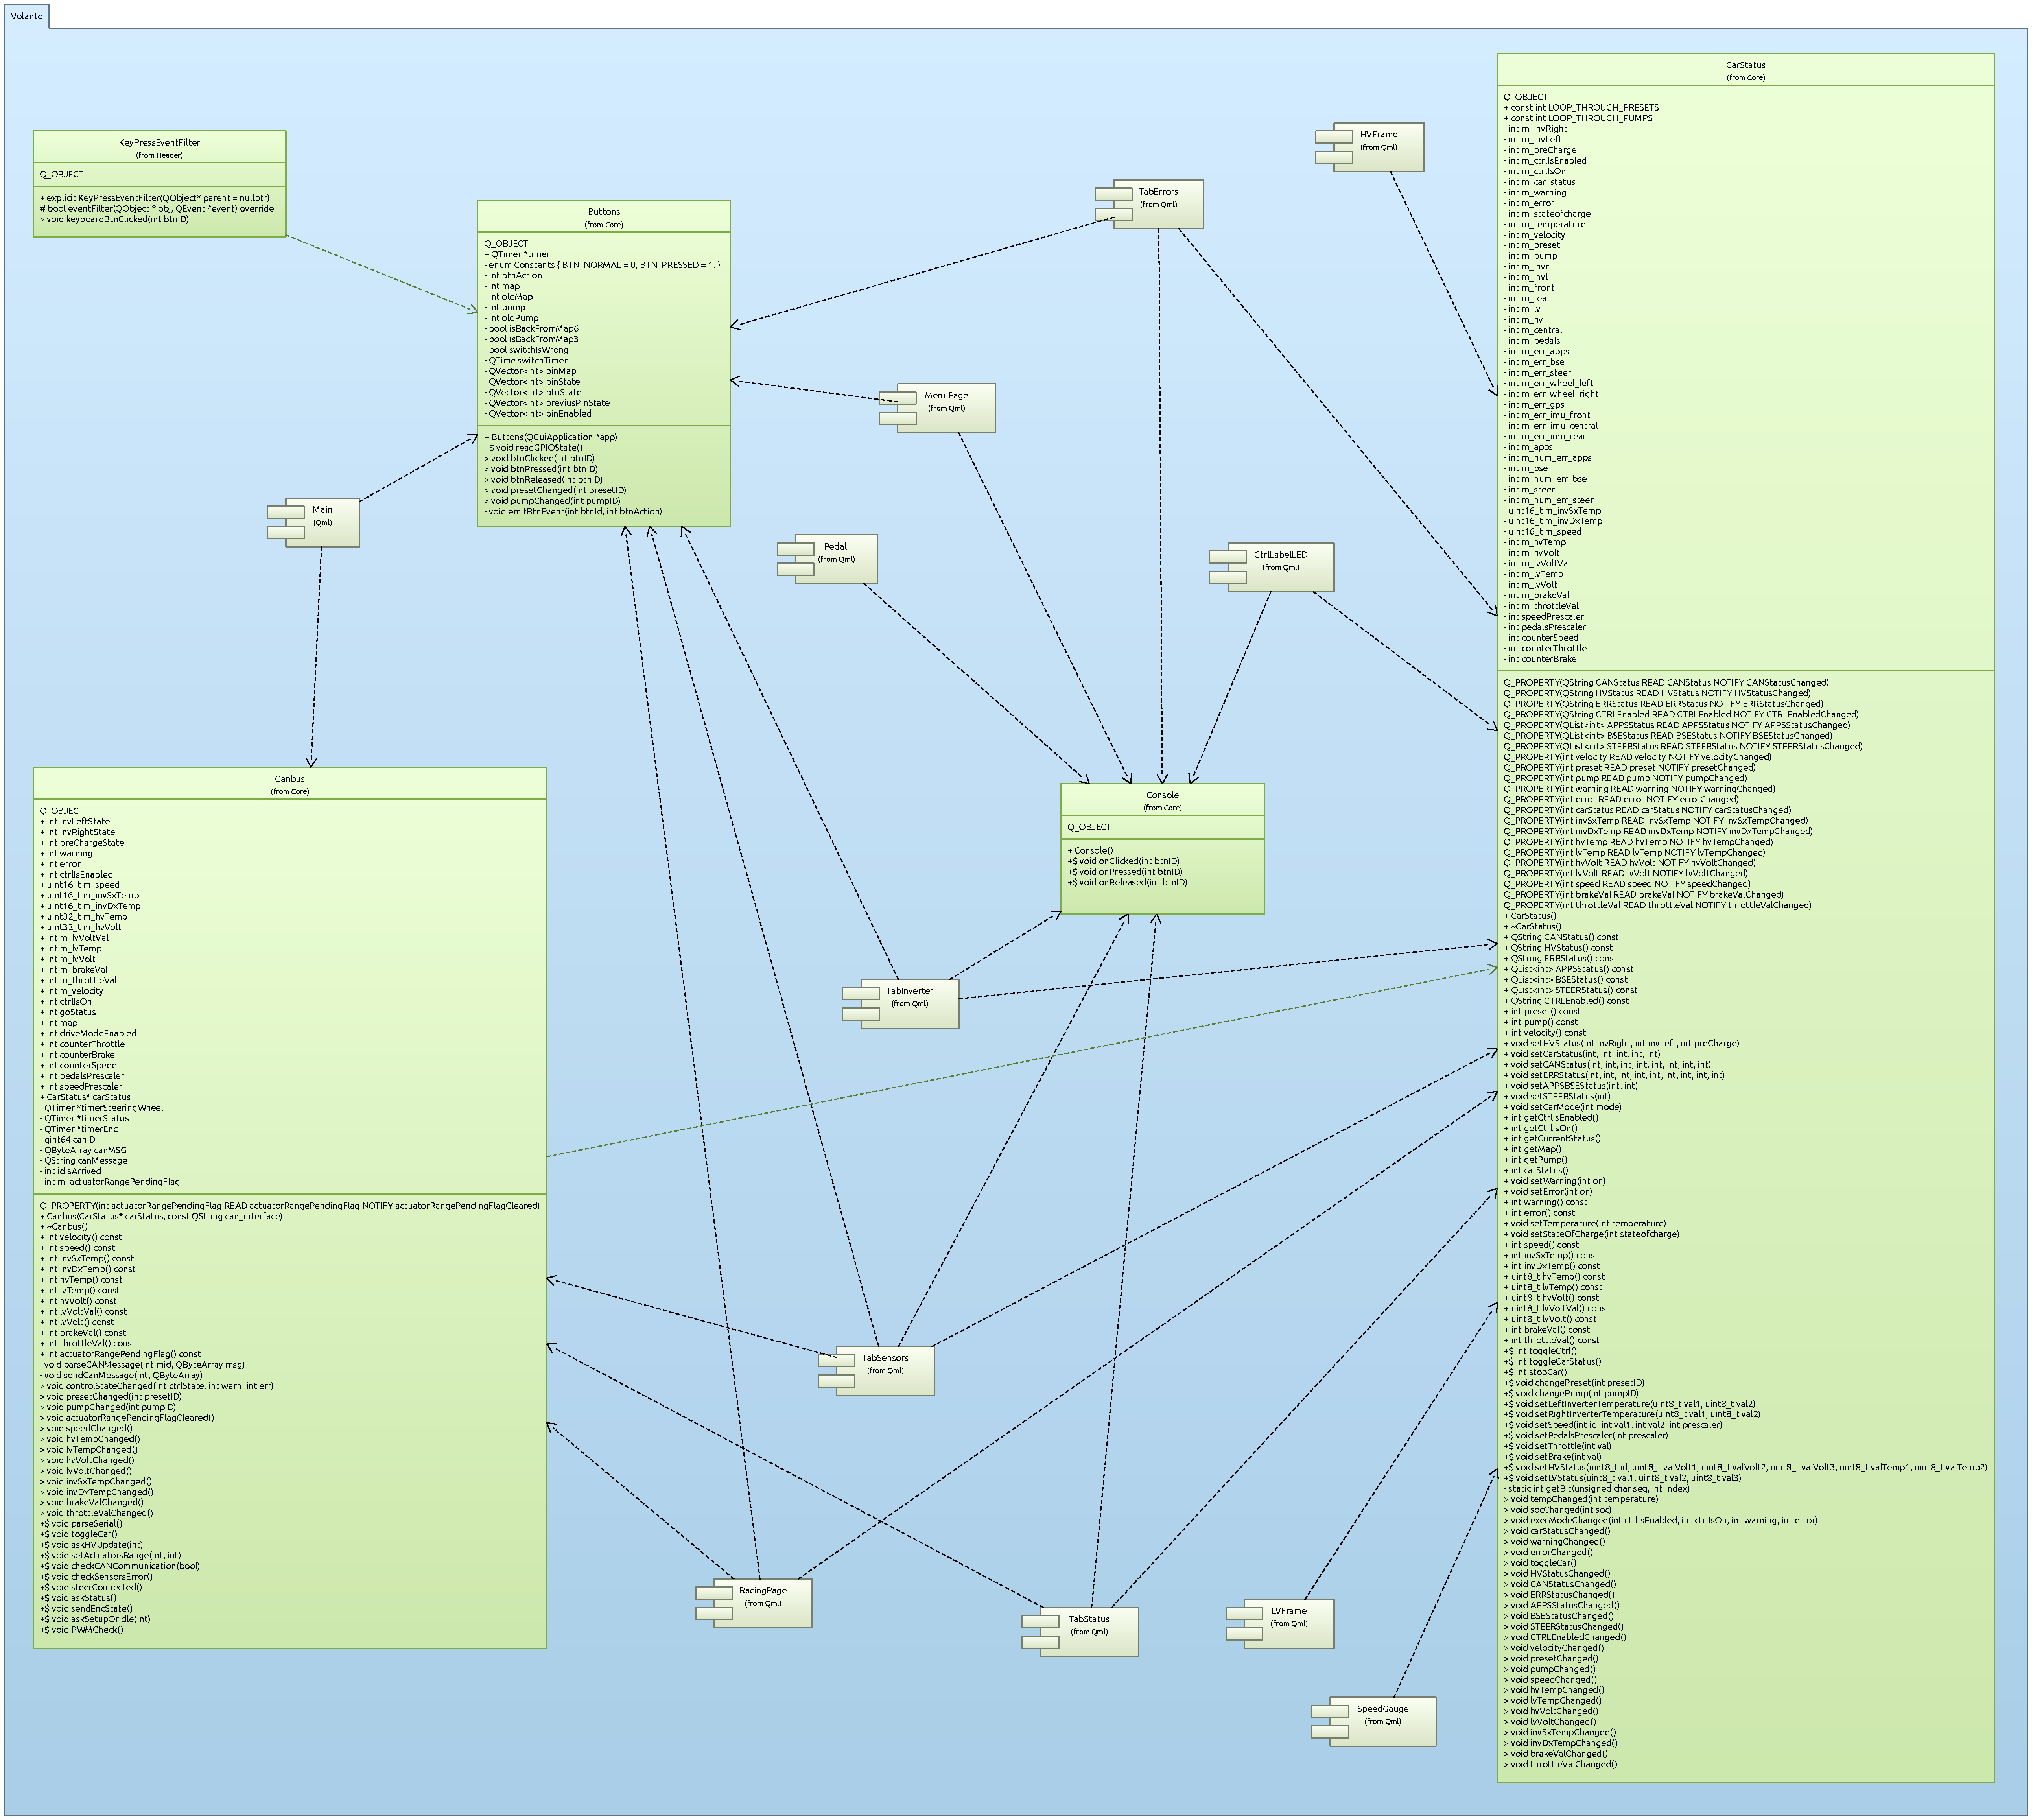
\includegraphics[width=0.75\textwidth]{./figures/cd.pdf}
    \caption{Class Diagram di Novembre 2018}
\end{figure}

Il progetto è composto da un file \emph{.pro} che ha come utilità quella di raggrupare tutte le componenti
del progetto, dai file compilabili \emph{.cpp} e \emph{.h} al \emph{qml.qrc}, che ci permette di raccogliere 
tutti gli assets principali, quindi immagini e i file \emph{.qml}.
Questo permette di mantere una struttura ordinata nella cartella del progetto e grazie al comando \emph{qmake},
che permette di generare il makefile specifico per la piattaforma in cui si sta facendo la build, permette di automatizzare 
tante procedure senza dover passare dal loro IDE proprietario. 
Durante lo sviluppo si è reso necessario documentare tutto il codice, perchè fino a quel momento non presentava commenti 
o guide in grado di spiegare le scelte prese e come funzionano alcune decodifiche dei messaggi, sia per il FE che per il BE. 
La repository inoltre mostrava difficolta nell'essere mantenuta quindi si è deciso di riorganizzare in sottocartelle e 
rimuovere le parti di codice non più utili in fase di test, soprattutto per la parte di qml in cui erano presenti pagine di prova e componenti
non più utilizzati.  

Il programa è diviso in tre parti:

\begin{itemize}
    \item La lettura dei dati dal Can-Bus (Canbus) 
    \item Lo stato della macchina (CarStatus)
    \item Il Front-End
\end{itemize}

% CanBus
La classe \emph{Canbus} si occupa di gestire l'invio e la ricezione dei messaggi via Can-Bus (SocketCan).
L'evoluzione, rispetto all'anno precedendete, è presente a lato hardaware, fornendo alla scheda la possibilità
di poter comunicare in Can-Bus direttamente, senza dover passare 
per una seriale e un dispositivo esterno visto come "gateway".
A livello software questo ha permesso di poter utilizzare la libreria 
di Qt basata sui driver Linux di cui ho già parlato.
Questa classe si occupa quindi di inviare messaggi quando richiesto dall'utente o in automatico, 
di ricevere e settare i valori nella classe \emph{CarStatus}.
% CarStatus
\emph{CarStatus} si occupa di salvare i valori letti precedentemente dal Can-Bus, 
in strutture dati in grado di essere lette dall'UI 
e se ritenuto necessario aggiornare l'interfaccia. 
Questo non era sempre presente nella versione precedente perchè essendo 
un prodotto in via di sviluppo non sempre questa scelta ci è sembrata la più veloce
dovendo aggiornare il codice in tempi brevi.
% QPROPERTY nel dettaglio
Il vanataggio di Qt è evidente quando si usano le sue librerie, 
in particolare se consideriamo l'aggiornamento di una digital dash la prima cosa che 
cambia notevolmente il workflow sono le sue \textbf{property}
che permetteno ai "meta-object" di poter comunciare tra di loro attravers il sistema \emph{signal} and \emph{slot}.
Le property si basano su funzioni per segnalare il cambiamento di un valore (NOTIFY), 
la sua lettura (READ), la sua scrittura (WRITE) e altre non utilizzate nel nostro caso. 
Questo permette di rendere accessibile un dato o una struttura dati dal Frontend al Backend 
e viceversa, in caso di input da parte dell'utente.
Il meccanismo inizialmente può sembrare macchinoso, poi, essendo mnemonico, può essere riutilizzato in molte 
situazione e, in termini di performance, permette di velocizzare l'accesso ai dati. 
Come introdotto precedentemente, senza conoscere il framework può sembrare più intuitivo utilizzare delle funzioni
in lettura e in scrittura pensate ad hoc, ma questa oltre a non essere la prassi influisce
sulle performance e in progetti grandi non permette di mantenere un'architettura precisa.
In termini di performance non sono stati fatti test mirati alla raccolta di dati sulla velocità di lettura e scrittura, 
ma abbiamo visto che alcuni valori non venivano letti soprattutto 
quando l'eseguibile è sotto stress per i continui messaggi Can-Bus.

\subsection{Interfaccia 2017}

% interfaccia con tab view d una pagina utilizzata in fase di run con info generiche, le altre con info specifiche
% si vedrà nel prossimo capitolo un approfondimento e come questa scelta sia stata riconsiderata

\begin{figure}[h!]
    \centering
    \begin{minipage}{0.5\textwidth}
        \centering
        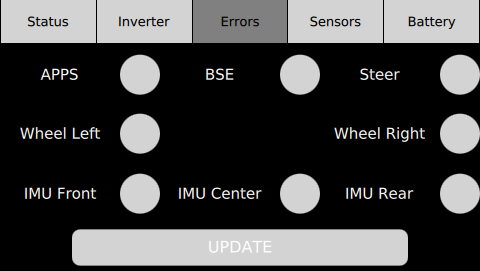
\includegraphics[width=0.8\textwidth]{./figures/oldUI/tabErrors.png}
        \caption{Interfaccia di Chimera - Tab View}
    \end{minipage}\hfill
    \begin{minipage}{0.5\textwidth}
        \centering
        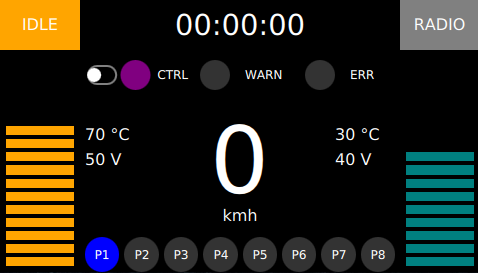
\includegraphics[width=0.8\textwidth]{./figures/oldUI/racingPage.png}
        \caption{Interfaccia di Chimera - Racing Page}
    \end{minipage}
\end{figure}

La digital dash di Chimera era stata pensata più in un ottica di test,
dividendo in due parti le funzionalità.
La prima parte, di configurazione e di lettura dello stato della sensoristica 
in una Tab View.
La Tab View necessitava principalmente di due tasti, uno per muoversi ed uscire dalla 
Tab e un altro per poter entrare e inviare il comando. Considerando il caso della \emph{Tab Errors} 
con il tasto in alto a sinistra è possibile spotarsi su quella vista, entrare con il tasto in basso a destra
e mandare il comando con lo stesso, per poi uscire con il tasto in alto a destra. 
La seconda parte, la \emph{Racing Page}, dove si poteva vedere lo stato di carica dei pacchi batteria,
i Kw erogati, lo stato della macchina e comunicare via radio con il muretto, funzione che non è mai stata implementata seriamente.
Nei prossimi capitoli verrà analizzata in modo più completo l'interfaccia e la \emph{Racing Page}, 
prendendo in considerazione le scelte fatte per Chimera Evoluzione.

\subsection{Finite State Machine}

\begin{figure}[hbt!]
    \begin{center}
        \begin{tikzpicture}[scale=0.2]
            \tikzstyle{every node}+=[inner sep=0pt]
            \draw [black] (40.5,-40.7) circle (3);
            \draw (40.5,-40.7) node {$Run$};
            \draw [black] (12.3,-22.1) circle (3);
            \draw (12.3,-22.1) node {$Idle$};
            \draw [black] (12.3,-22.1) circle (2.4);
            \draw [black] (67.9,-22.1) circle (3);
            \draw (67.9,-22.1) node {$Setup$};
            \draw [black] (15.3,-22.1) -- (64.9,-22.1);
            \fill [black] (64.9,-22.1) -- (64.1,-21.6) -- (64.1,-22.6);
            \draw [black] (65.42,-23.78) -- (42.98,-39.02);
            \fill [black] (42.98,-39.02) -- (43.92,-38.98) -- (43.36,-38.15);
            \draw [black] (42.98,-39.02) -- (65.42,-23.78);
            \fill [black] (65.42,-23.78) -- (64.48,-23.82) -- (65.04,-24.65);
            \draw [black] (64.9,-22.1) -- (15.3,-22.1);
            \fill [black] (15.3,-22.1) -- (16.1,-22.6) -- (16.1,-21.6);
            \draw [black] (38,-39.05) -- (14.8,-23.75);
            \fill [black] (14.8,-23.75) -- (15.2,-24.61) -- (15.75,-23.77);
        \end{tikzpicture}
    \end{center}
    \caption{Finite State Machine del Volante}
\end{figure}

Il funzionamento della macchina a stati del Volante è gestita dall'ECU. 
La FSM rispecchia il lavoro del Team del Controllo, lo scopo del Volante è quello di permettere al pilota 
di poter cambiare, in sicurezza, lo stato. In sicurezza perchè la maggior parte dei controlli avvengono lato ECU
e il Volante è stato sviluppato per rendere il più intuitivo e a prova di errori umani la procedura di accensione. 
Tramite l'interfaccia possiamo inviare richieste e se sono accettate dall'ECU, quindi se è possibile cambiare stato dallo stato di partenza,
effettua i controlli e le richieste a chi di dovere e risponde in modo positivo.
La monoposto, successivamente all'accensione del pacco low voltage (BMS LV) si troverà in \textbf{IDLE}, 
da qui se non si presentano errori si può mandare una richiesta di \textbf{START} 
e se la risposta è positiva possiamo quindi passare alla fase di \textbf{SETUP}. 
Durante questa richiesta l'ECU si occuperà di chiedere al pacco high voltage (BMS HW) di accendersi chiudendo in serie il primo e il secondo AIR. 
Se l'accensione termina con successo il BMS HV risponde all'ECU, la quale poi conferma al Volante lo stato Setup.
Il pilota ora ha due possibilità: richiedere l'accensione degli Inverter, e se questa procedura termina correttamente
sarà possibile mandare una richiesta per entrare nella fase di \textbf{RUN}, in cui l'ECU abilita l'utilizzo della pedaliera.
Oppure mandare una richiesta di spegnimento del pacco batteria high voltage attraverso il comando di \textbf{STOP}.
Il Volante ha due possibilità quando si trova in RUN: 

\begin{itemize}
    \item Errori: In base al tipo di errore che riscontra l'ECU può fare richiesta di spegnimento al pacco low voltage o passare in fase di IDLE.
    \item SetUp: Richiesto dal pilota, disabilita la pedaliera e bisogna ripetere la procedura di accensione degli inverter. 
\end{itemize} 

Bisogna sempre tenere in considerazione che le variabili di stato che vengono modificate dipendono
dai messaggi presenti nella rete e che hanno come destinario il Volante, dovendo sempre ricevere un feedback da parte dall'ECU
L'utente, che sia il pilota o chi sta testando la macchina, ha poche responsabilità in caso di errore.
Gli errori che si possono riscontrare sono da verificarsi nei cambiamenti di stato o negli stati stessi della FSM e dalle componenti
della monoposto per possibili malfunzionamenti.  
Solo i manettini, per come è stato scritto il codice, permettono di aggiornare l'interfaccia senza ricevere un feedback
in quanto il messaggio sullo stato di connessione del Volante è inviato in ogni 500ms, si per mostrare la presenza nella rete
che per condividere le preferenze del pilota.


\newpage


\subsection{Cross Compilazazione}


\begin{figure}[hbt!]
    \centering
    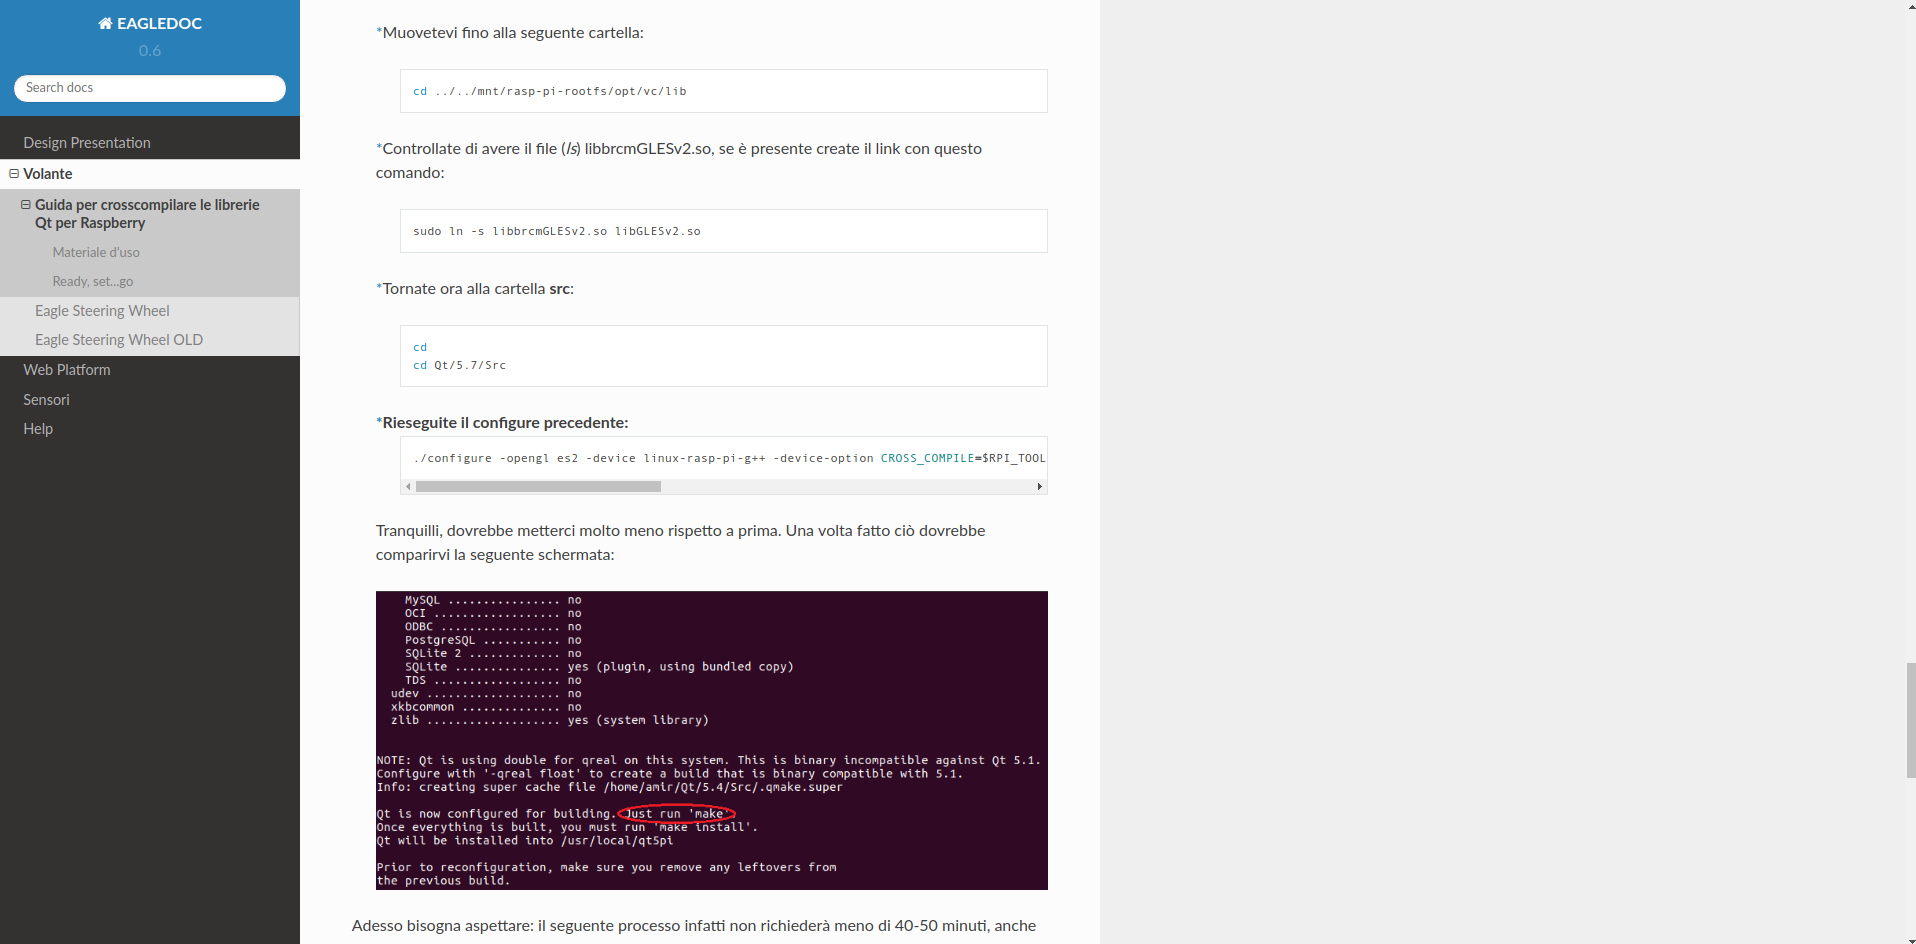
\includegraphics[width=0.75\textwidth]{./figures/cross-compilazione.png}
    \caption{Guida Cross Compilazione del Team \cite{cross-compilazione}}
\end{figure}


% APPROCCIO ALLO SVILUPPO SUL SISTEMA EMBEDDED

L'approcio allo sviluppo del progetto si è diviso in due parti.
La prima parte è stata buildare il progetto sul laptop ed eseguirlo, 
cambiando la classe bottoni per poter avere gli input da tastiera e utilizzare 
una interfaccia virtuale per la comunicazione Can-Bus.
Per l'utilizzo dei bottoni si è deciso di mantenere la posizione de tasti del Volante portandoli sulla tastiera.
I quattro tasti funzione sono disposti a "quadrato" sono diventati "Q-A-D-R", 
per il manettino delle mappe invece sono stati utilizzati i numeri fino al 6.
Per quanto riguarda invece gli altri due manettini i test sono stati fatti via \emph{ssh} valutando l'input 
e il loro cambiamento di stato, successivamente sono stati portati anche loro su tastiera usando in ordine 
le lettere della parte destra della tastiera quindi per le pompe "T-Y-U-I-O-P" e per il controllo "F-G-H-J-K-L".    
La seconda parte ci ha messo più in difficoltà perchè inizialmente abbiamo avuto problemi di compatibilità 
con il sistema operativo del target device e la sua versione di Qt che non risultava congruente con la nostra.
Precedentemente il Volante era stato compilato con la versione 5.7 di Qt, con il nuovo sistema operativo, buildato
con Buildroot, potevamo installare solamente la 5.10.1. 
Questo inizialmente è apparso come un problema da poco ma quando abbiamo visto che per una classe, \emph{QCanBus}, 
le funzioni non erano più presenti nello stesso modo abbiamo dovuto rivedere la procedura di cross-compilazione per
riuscire a compilare il codice con la versione successiva di Qt. 
Allineate queste divergenze, gli approcci che abbiamo considerato cercando nella documentazione di Qt e nei forum
sono due:

\begin{itemize}
    \item Deploy su Target Board
    \item Deploy in Locale 
\end{itemize}

Noi abbiamo deciso di compilare il progetto dal nostro host e poi spostare l'eseguibile sul target device, automatizzando la procedura attraverso 
uno script in bash utilizzando l'auto-login di \emph{ssh}, il kill del processo in esecuzione per poi poter trasferire la versione appena compilata ed eseguirla.
La scelta è motivata dal poter lasciare il target device più leggero e non avere necessità di esso nella fase di compilazione, ma solo per eseguirlo.
Per compilare il codice del Volante da un dispositivo linux abbiamo dovuto cross-compilare, 
questo significa che mediante un compilatore esterno abbiamo "emulato" il sistema target compilando il sorgente 
come se fossimo l'host di riferimento. Così da poter eseguire il file su un architettura diversa da quella del host di origine.
Questa è stata la difficoltà più grande riscontrata con l'utilizzo di Qt per dispositivi ARM, abbiamo dovuto trovare il modo di testare 
in locale l'applicazione, senza avere a disposizione il dispositivo. 
La procedura per avere l'ambiente adatto a cross-compilare, considerata la versione open-source e
non fornendo la tool-chain proprietaria, è molto lenta e richiede ore per poterla portare a termine.
La guida che abbiamo ottenuto prevede il montare il sistema operativo del target device (in questo caso non lo stesso, ma raspbian lite) 
e installare le librerie di Qt, per poi avere il qmake necessario a generare il makefile adatto allo scopo.

% Conclusioni sulla cross-compilazione

La nostra inesperienza nel settore ci ha fatto impiegare molto tempo nella risoluzione 
di problemi anche banali, ma ci ha anche permesso di imparare tanto e soprattutto di capire
che esistono soluzioni più semplici, ancora da testare, delle quali parlerò meglio nelle valutazioni.

\section{Redesign della Applicazione}

% problemi dell'interfaccia a livello software e come sono stati risolti 
% disegno su carta con low fidelity prototype --> mockup

L'utilizzo del Framework Qt ha portato numerosi vantaggi quando è stato deciso di ridisegnare l'interfaccia.
Inizialmente gli oggetti che componenvano la UI erano tutti nel meta linguaggio \emph{QML} utilizzato da Qt, questi oggetti si basano 
sul linguaggio JavaScript e permettono di attribuire proprietà all'interfaccia per poi essere gestita dagli eventi generati dal codice C++.
Questo in partenza è risultato essere un limite quando si è deciso di utilizzare il formato \emph{.png} per comporre la strumentazione, 
ma successivamente abbiamo riscontrato la predisposizione di Qt all'utilizzo di immagini.

\subsection{Dal Low Fidelity Prototype al primo Mockup}

Tutto è iniziato da un foglio di carta, un A3 per la precisione, dopo aver raccolto tutti requisti da parte del team
abbiamo iniziato a disegnare e a pensare come poteva essere aggiornato il Volante per venire incontro alle nostre necessità.

Le persone coinvolte nel redesign dell'applicazione sono state:

\begin{itemize}
    \item Davide Farina: Pilota e quindi primo utilizzatore del Volante
    \item Luca Martinelli: Sviluppatore e utilizzatore del Volante come debugger per la macchina
    \item Laura Scoccianti Designer, che si è occupata di portare l'interfaccia da Low Fidelity Prototype a Mockup 
\end{itemize}


\begin{figure}[hbt!]
    \centering
    \includegraphics[width=0.75\textwidth]{./figures/lowfidelityprototype.jpg}
    \caption{Low Fidelity Prototype}
\end{figure}

% disegno

% cosa abbiamo deciso quindi? cornice hv e lv sempre presenti, ridimensionamento oggetti non necessari

Il Low Fidelity Prototype ha preso subito forma, ed una delle cose che è stata in primo luogo fatta presente è
la possibilità di potersi muovere in modo intuitivo nelle Tab, quindi senza dover passare da una vista Tab View a una pagina singola
come era in precedenza.
La giustificazione nasce dall'esigenza di una migliorare usabilità, in quanto anche in fase di \emph{RUN} deve essere possibile cambiare Tab.
Questo ha fatto si che la \emph{Racing Page} dovesse essere integrata nella vista a Tab oppure di cambiare completamente layout.
Una delle prime proposte è stata la visuale dello stato della macchina in tutte le pagine, insieme al livello di carica dei due pacchi 
batteria. Questo ci ha messo davanti ad una scelta, integrare questi indicatori all'interno di ogni pagina o utilizzarli come cornice. 
La seconda scelta si è rivelata la più efficace e semplice da implementare, senza dover badare alla riscrittura di codice in più parti.
Un'altra funzionalità, che a livello estetico ha permesso di "animare" l'interfaccia
in fase di test con il tractive system disattivato, è stata l'inserimento di due slider per i sensori della pedaliera.
L'accelleratore e il freno nella Racing Page del Volante sono stati pensati per poter dare un feedback sulla pressione completa, quindi quando 
si è al 100\% durante l'accellerazione.  
Una proposta che è stata poi scartata è stata la possibilità di visualizzare in una Tab dedicata la dinamica del veicolo potendo
valutare la \emph{g-force} letta dalle IMU, l'implementazione si basava su un grafico a radar stile Formula 1.

Per quanto riguarda la scelta di stile e colori da utilizzare per l'interfaccia ci siamo ispirati al mondo della Formula E
e dei videogiochi Racing, utilizzando colori molto accesi e facili da distinguere anche in situazioni di scarsa luminosità.
Questo è uno dei punti forte della nostra interfaccia, la cura dei particolari e soprattutto la scelta dei colori è 
stata molto discussa dovendo mostrare e far percepire al pilota in breve tempo il cambiamento di certe condizioni.  

Ognuna delle persone coinvolte ha dato la sua opinione sulla fattibilità delle funzioni da integrare e sulla loro utilità
votando su quali erano da mantenere e altre da scartare o mettere come ultime nel processo di integrazione.
Così facendo si è definito il Gantt per l'integrazione delle funzionalità. 

Successivamente è stato necessario portare questo prototipo in qualcosa di più definitivo e integrabile nell'interfaccia.
Il risultato è stato reso possibile da Laura Scoccianti, che si è da sempre occupata della parte grafica del team, in questo caso 
ha portato il nostro Low Fidelity Prototype in un High Fidelity Prototype utilizzando un software per la grafica.
Elaborato il primo mockup, dopo averne discusso con i membri del Team siamo passati all'integrazione, ogni singola parte della UI
è stata poi esportata in formato \emph{.png} e integrato con le funzioni già presenti e in corso di sviluppo della macchina. 

Questo tipo di approccio è stato reso possibile dalla definizione già in partenza della composizione del team e delle task
e basando il processo di sviluppo sui clienti interni ed esterni visti come il "pilota", il "tester" e chi si è occupato della realizzazione.

\subsection{Integrazione della nuova UI del Volante}

% probelma della cornice - risolta rendendo la tab view più piccola ed eliminando i nomi delle tab, mostrando solo come indicatore su quale tab si è
% integrazione dell'accelleratore freno nella racing page
% utilizzo dei paddle per potersi muovere più agevolemente nell'interfaccia e aumentare le funzionalità dei quattro tasti sulla maschera frontale
% aprendo al'integrazione di funzioni come pressione di più tasti insieme

\begin{figure}[hbt!]
    \centering
    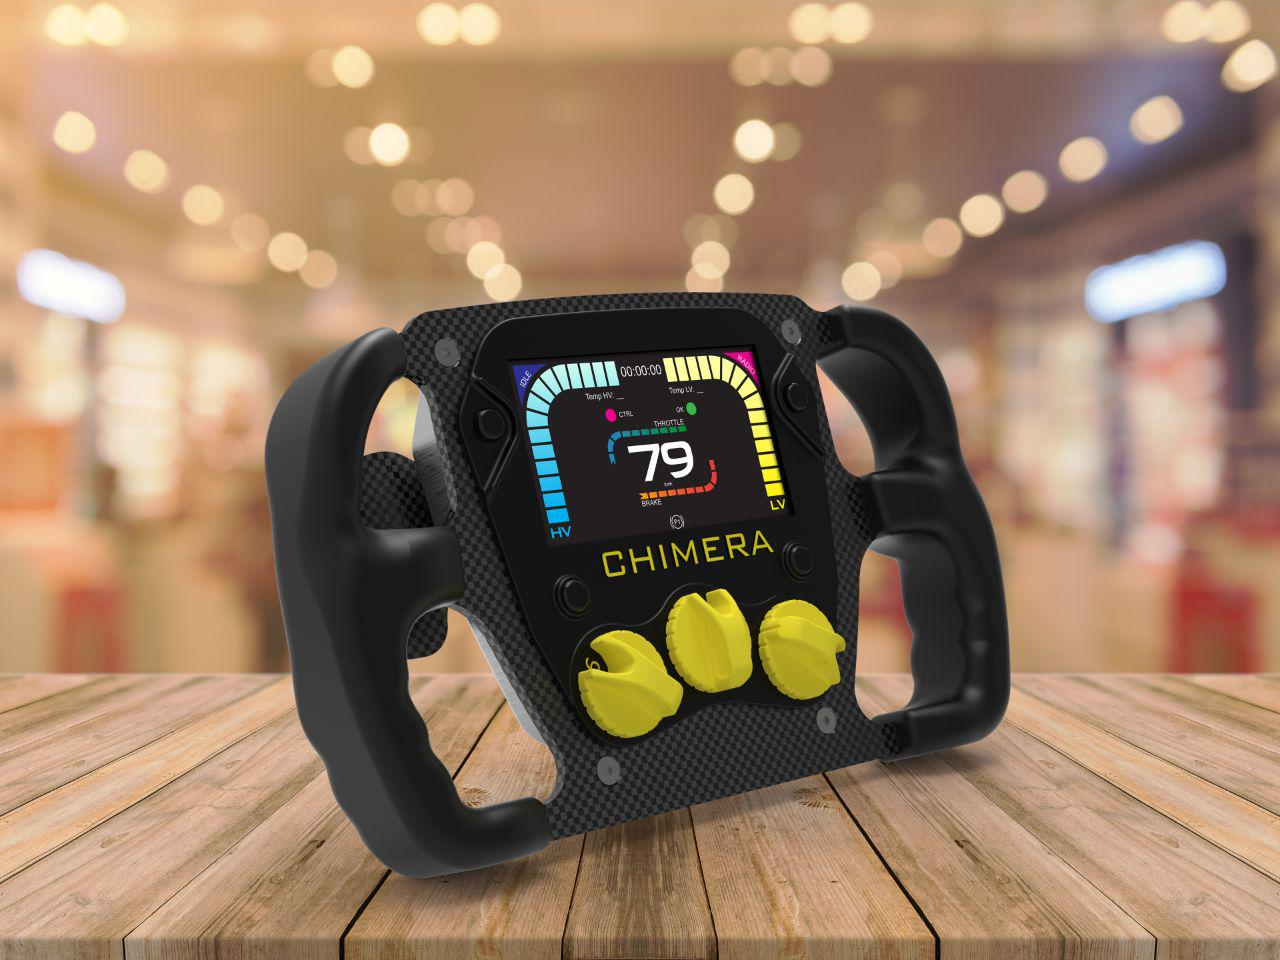
\includegraphics[width=0.75\textwidth]{./figures/primoMockUpUI.jpg}
    \caption{Primo Mockup}
\end{figure}

% integrazione della cornice
Il problema della cornice da integrare è stato risolto ridimensionando la Tab View per fare spazio 
agli indicatori del pacco HV,LV e inserendo il timer non ancora implementato su Chimera. 
L'integrazione ha dato problemi nello sviluppo perchè la UI non era mai stata pensata per essere reponsive, in quanto in un ambito come questo non 
è effettivamente richiesto. 
Le difficoltà sono apparse nel dover integrare le funzioni per gestire il valori da visualizzare inserendoli allo stesso livello nel \emph{main.qml}
Tab e corince.
% orientamento posizione tab
Il ridimensionamento delle Tab ha portato alla perdita della visualizzazione del nome della Tab in cui si è, fattore molto importante
perchè la mancanza di riferimenti durante l'utilizzo del programma peggiora l'esperienza d'uso.
La soluzione è stata indicare la posizione delle Tab nella parte inferiore del display e, grazie l'utilizzo dei paddle, sapere se bisogna andare a destra o a 
sinistra per visualizzare la Tab desiderata. 
In più prima non era possibile tornare indietro nelle Tab ma si potevano percorrere solo da sinistra verso destra.
Questo fa parte dei compromessi che non si sono rivelati negativi, anzi l'interfaccia di Chimera Evoluzione nasce dalle mancanze riscontrate da Chimera.
Una nota sull'interfaccia risulta doverosa, questo non è un dispositivo adatto e utilizzato da tutti, ma solo da chi è stato istruito 
sul funzionamento della macchina e sulla sua parte elettronica. I nostri piloti sono all'interno del team e lavorano con noi
allo sviluppo della monoposto.

\begin{figure}[h!]
    \centering
    \begin{minipage}{0.5\textwidth}
        \centering
        \includegraphics[width=8cm]{./figures/imageracing.jpg} % first figure itself
    \end{minipage}\hfill
    \begin{minipage}{0.5\textwidth}
        \centering
        \includegraphics[width=8cm]{./figures/imagetutorial.jpg} % second figure itself
    \end{minipage}
\end{figure}

% pedaliera
L'integrazione dei sensori della pedaliera nella \emph{Racing Page} invece non ha riscontrato particolari problemi, è stata rideimensionata la
grandezza del rettangolo in cui dovevano essere collocati i \emph{.png} che hanno mantenenuto le dimesnioni del display (il layer in questo caso)
quando sono state esportate è stato solo macchinoso farli risultare nella posizione corretta durante l'aggiornamento dei KW.
Questo ha anche permesso di rivalutare la grandezza dei font e, verificando direttamente con il pilota, la nostra grafica ci ha fornito i file con le dimensioni
aggiornate che si è trattato solo di ri-integrare nella interfaccia.
% velocità
Un'altra integrazione, dovuta all'aggiunta degli encoder sulle ruote, è stato il calcolo della velocità, oltre al valore dei KW richiesti ora
è possibile visualizzare in \emph{Racing Page} anche la velocità calcolata dalle schede che si occupano della sensoristica.
% radio-feedback
Il sistema di comunicazione radio, che è stato lentamente abbandonato nel corso dello sviluppo della monoposto, ha lasciato spazio, utilizzando
il suo tasto in alto a destra nell'interfaccia, all'invio di un marker in CAN che permette al pilota di segnalare in un certo momento che è successo 
qualcosa.
% calibrazione pedaliera
Durante lo sviluppo si è reso necessario integrare una procedura per calibrare la pedaliera, questo ha messo in risalto alcune criticità 
nel come era stata pensata la UI mostrando possibili approcci diversi.
La calibrazione è stata implementata potendo muoversi nei vari sensori con una procedura interattiva segnalando all'utente se ha effettivamente
concluso una delle fasi. Le criricità sono apparse nel momento in cui bisognava mostrare il feedback, cambiando solamente il testo a volte non si permette all'utente 
di accorgersi se ha effettivamente concluso quella parte. Il problema è stato preso e analizzato e le soluzioni saranno visibili nella prossima implementazione
del Volante per la stagione 2019/2020.  







\newpage






\section{Funzionalità delle diverse pagine}

% spiegazione struttura grafica della pagina, per poi finire nella racing page

L'interfaccia del Volante di Chimera Evoluzione è composta da più Tab disposte in serie che permettono di seguire in ordine
la procedura di accensione e di test standard della monoposto. Alcune funzionalità sono state inserite solo a livello grafico
e per dare forma all'interfaccia, sono state successivamente implementate su Chimera Evoluzione. 
I nomi delle Tab hanno subito modifiche perchè per come era stata concepita non erano presenti 
vere relazioni tra il nome, le funzionalità e ciò che doveva essere visualizzato. 
La versione mostrata è quella standard utilizzata per i test. 

\subsection{Warning Tab}

\begin{figure}[h!]
    \centering
    \begin{minipage}{0.5\textwidth}
        \centering
        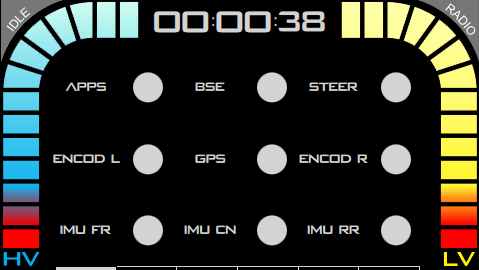
\includegraphics[width=0.9\textwidth]{./figures/UI/tabWanings.png}
        \caption{Chimera Evoluzione - Tab Warnings}    
    \end{minipage}\hfill
    \begin{minipage}{0.5\textwidth}
        \centering
        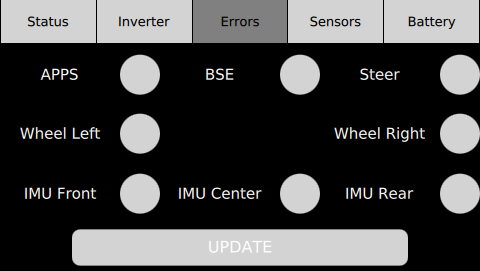
\includegraphics[width=0.9\textwidth]{./figures/oldUI/tabErrors.png}
        \caption{Chimera - Tab Errors}
    \end{minipage}
\end{figure}

La prima Tab, chiamata anche \emph{Warning Tab}, mostra lo stato della sensoristica.
Diversamente dalla \emph{Errors Tab}, i warnings non sono errori critci e servono 
solo a informare il pilota se certi sensori non funzioneranno come dovrebbero.
Inizialmente erano presenti alcuni sensori che sono stati rimossi perchè non più necessari,
e la richiesta di update è stata resa automatica per poter aumentare lo spazio nella Tab.  
Nelle prime fasi di test questa funzionalità si è rivelata molto utile perchè ci ha permesso
di vedere sin dalla prima accensione se i dispositivi erano collegati e funzionavano.
Con la presenza di warnings è possibile abilitare il tractive system e utilizzare la macchina, 
se dovessero apparire degli warnings durante la fase di \emph{Run} questo non non cambierebbe lo stato,
cosa che invece accade per gli errori.

\subsection{Error Tab}

\begin{figure}[h!]
    \centering
    \begin{minipage}{0.5\textwidth}
        \centering
        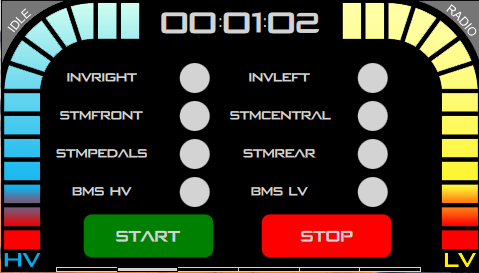
\includegraphics[width=0.9\textwidth]{./figures/UI/tabErrors.png}
        \caption{Chimera Evoluzione - Tab Errors}    
    \end{minipage}\hfill
    \begin{minipage}{0.5\textwidth}
        \centering
        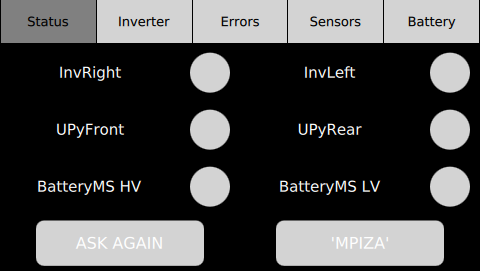
\includegraphics[width=0.9\textwidth]{./figures/oldUI/tabStatus.png}
        \caption{Chimera - Tab Status}
    \end{minipage}
\end{figure}

La seconda Tab, chiamata anche \emph{Errors Tab}, permette di visualizzare la panoramica degli errori presenti in macchina, 
se sono presenti errori critci andranno verificati con gli interessati e risolti per poter entrare nella fase di \emph{Setup}.
In questa Tab è stata ripensata la procedura di accensione, cambiando il comando di \emph{Ask Again} con il comando di \emph{Stop}
ed è stata ridimensionata per poter inserire altre scheda come ad esempio la pedaliera.
Se non sono presenti errori, possiamo mandare il messaggio di \emph{Start} e successivamente poter tornare nella fase \emph{Idle}
tramite il comanodo \emph{Stop}.


\newpage


\subsection{Status Tab}

\begin{figure}[h!]
    \centering
    \begin{minipage}{0.5\textwidth}
        \centering
        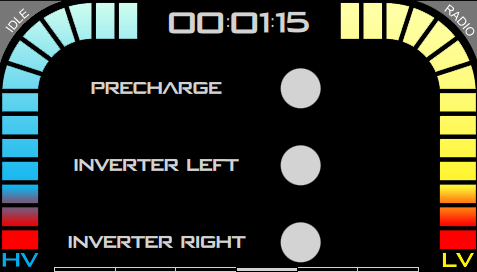
\includegraphics[width=0.9\textwidth]{./figures/UI/tabStatus.png}
        \caption{Chimera Evoluzione - Tab Status}    
    \end{minipage}\hfill
    \begin{minipage}{0.5\textwidth}
        \centering
        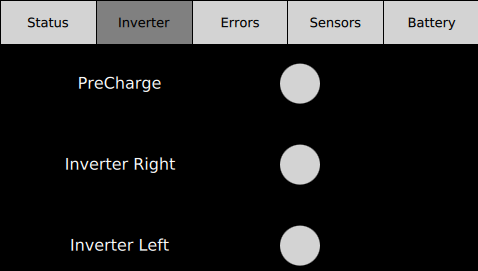
\includegraphics[width=0.9\textwidth]{./figures/oldUI/tabInverter.png}
        \caption{Chimera - Tab Inverter}
    \end{minipage}
\end{figure}

La terza Tab, chiamata anche \emph{Tab Status}, mostra lo stato della precharge e degli inverter.
Da qui, grazie ai led, possiamo vedere se non comunicano, quindi led grigio, se sono abilitati o no (rosso e verde).
Questa Tab permette di accendere o spegnere gli inverter facendone richiesta.
Questa procedura deve essere effettuata prima di entrare nella \emph{Racing Page} per poter entrare nella modalità \emph{Ready To Drive}.
Non è possibile entrare in questa modalità, se non vengono abilitati, in quanto di default sono impostati ad off.

\subsection{Racing Page}

\begin{figure}[h!]
    \centering
    \begin{minipage}{0.5\textwidth}
        \centering
        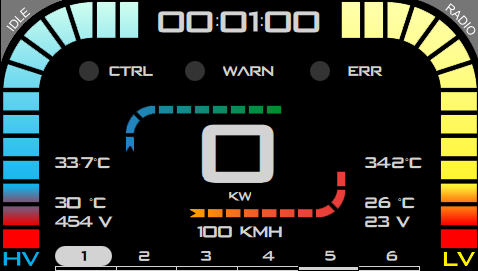
\includegraphics[width=0.9\textwidth]{./figures/UI/racingPage.png}        
        \caption{Chimera Evoluzione - Racing Page}    
    \end{minipage}\hfill
    \begin{minipage}{0.5\textwidth}
        \centering
        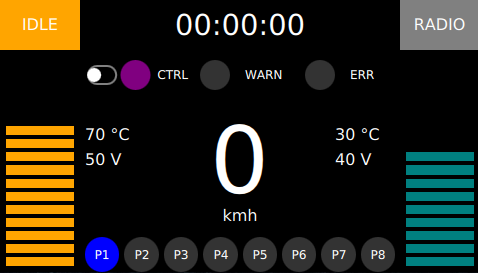
\includegraphics[width=0.9\textwidth]{./figures/oldUI/racingPage.png}
        \caption{Chimera - Racing Page}
    \end{minipage}
\end{figure}

La quarta Tab, chiamata anche \emph{Racing Page} è la più importante e la più curata dal punto di vista del design.
Senza doversi spostare in altre Tab si è in grado di avere una visione generale della macchina.
Da qui si può interagire con la sezione in alto a sinistra che mostra lo stato della macchina (idle, setup, run, stop)
attraverso il comando di \emph{Run} e il relativo comando di \emph{Stop} che nel primo caso abilitano l'utilizzo della pedaliera
e nel secondo permettono di tornare nella fase di \emph{Setup}, disabilitando gli inverter.
Nella parte più alta sono presenti tre led che mostrano se il controllo è stato abilitato e in sequenza 
i possibili warning o errors presenti in macchina in caso di malfunzionamenti durante la fase di \emph{Run}.
L'introduzione di questi led è stato inoltre utile per evitare che il pilota possa entrare, se non abilitato, nella fase di \emph{Run}
tenendo sempre a mente che il Volante non si occupa di gestire i casi di errore, ma solo di visualizzarli.
Le funzioni disponibili, come già spiegato, sono definite dalla macchina a stati.
Al centro dello schermo è posizionato il valore, in KW, richiesto ai motori, 
attorno possiamo trovare in azzuro quanto viene premuta la pedaliera e in rosso lo stato del freno per dare un feedback al pilota 
mostrandogli, in accellerazione, quando si trova al 100\%.
Appena sotto invece è posizionata la velocità letta dagli encoder, fino ad arrivare alla mappa scelta.
In questa sezione il pilota può vedere in che mappa si trova, scelta grazie all'ausilio dei manettini.
Le mappe permettono di selezionare, in \%, la potenza da erogare ai motori, la prima mappa abilita la retromarcia (-20\%), 
dalla seconda in poi invece incrementa del 20\% fino ad arrivare alla mappa 6 che indica il massimo erogabile.  
Il selettore delle mappe oltre ad essere molto utile in fase di test, soprattutto per verificare in linea generale la sicurezza della macchina 
apre molte possibilità in termini di personalizzazione della guida. 
Il pilotta infatti oltre a questo manettino ne ha a dispozione altri due: uno per impostare il traction control e l'altro per il sistema di cooling. 
Grazie al primo il pilota può decidere se abilitare il torque vecoring, disattivarlo e utilizzare o no lo slip control e con l'ausilio del secondo
può impostare, manualmente, l'utilizzio delle pompe che indipendentemente da questo funzionano autonomamente.    
Rispettivamente sulla parte sinistra e destra troviamo lo stato del pacco lov voltage e high voltage con le loro temperature e voltaggio.
In più, durante la fase di test, si è reso necessario mostrare la temperatura degl inverter, da cui si è deciso di inserire questi dati 
congruentemente alla posizione degli inverter in macchina, quindi sinistra per l'inverter di sinistra e destra per l'inverter di destra.

\subsection{Battery Tab}

\begin{figure}[h!]
    \centering
    \begin{minipage}{0.5\textwidth}
        \centering
        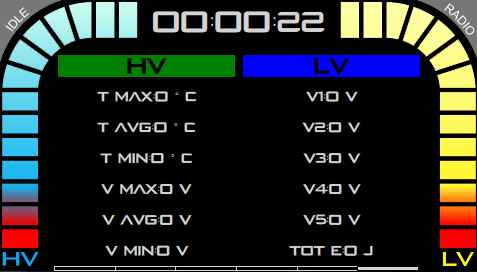
\includegraphics[width=0.9\textwidth]{./figures/UI/tabBattery.png}
        \caption{Chimera Evoluzione - Tab Battery}    
    \end{minipage}\hfill
    \begin{minipage}{0.5\textwidth}
        \centering
        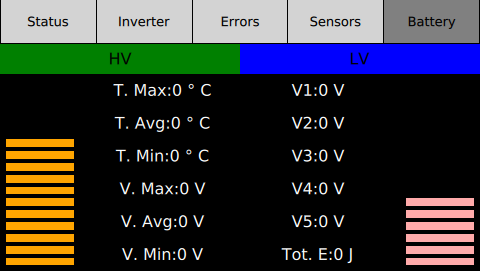
\includegraphics[width=0.9\textwidth]{./figures/oldUI/tabBattery.png}
        \caption{Chimera - Tab Battery}
    \end{minipage}
\end{figure}

La quinta Tab, chiamata anche \emph{Battery Tab}, permette di visualizzare lo stato di carica del pacco batterie High Volage e Low Voltage.
Per entrambe è presente la temperatura minima, massima e media della temperatura e della carica dei due pacchi.
Questa Tab è da utilizzare in fase di test, in quanto al pilota non avrà, o solo in pochi casi particolari, 
la necessità di sapere lo stato delle celle. Le informazioni più generali sono presenti invece nella \emph{Racing Page}.  


\subsection{Sensor Tab}

\begin{figure}[h!]
    \centering
    \begin{minipage}{0.5\textwidth}
        \centering
        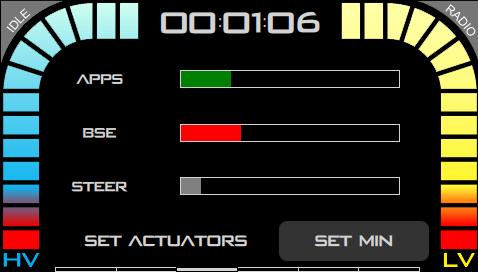
\includegraphics[width=0.9\textwidth]{./figures/UI/tabSensors.png}        
        \caption{Chimera Evoluzione - Tab Sensors}    
    \end{minipage}\hfill
    \begin{minipage}{0.5\textwidth}
        \centering
        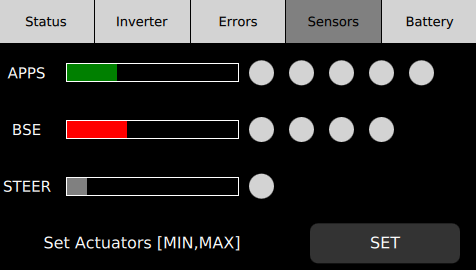
\includegraphics[width=0.9\textwidth]{./figures/oldUI/tabSensors.png}
        \caption{Chimera - Tab Sensors}
    \end{minipage}
\end{figure}

La sesta Tab, chiamata anche \emph{Tab Sensori}, è composta dai valori raccolti dalla pedaliera e dallo sterzo (APPS, BSE and STEER).
In questa Tab è possibile vedere attraverso una barra orizzontale che valori assumono, in modo indicativo, i sensori di riferimento.
La pedaliera è composta dall'acceleratore e dal freno, che come già spiegato, in una scala da 0 a 10 sono visualizzabili anche nella \emph{Racing Page}.
Per tutti e tre i sensori si è reso necessario l'implementazione di una procedura di calibrazione, 
nella quale il pilota o chi testa la sensoristica è in grado di far memorizzare il valore massimo e minimo alle schede di riferimento.
Questa procedura ci è stata molto utile durante i test ed essendo interattiva è anche facile da seguire. 


\newpage


\section{Considerazioni sullo Sviluppo dell'Interfaccia}

Il lavoro che è stato fatto ha messo al centro dello sviluppo il cliente, considerato nel nostro caso il pilota e 
i suoi utilizzatori che lo vedono come strumento di debug, che è stato da sempre membro attivo durante lo sviluppo.
La metodologia utilizzata ha permesso di migliorare l'usabilità mostrando un'attenzione particolare per il punto estetico 
e rafforzare la flessibilità del prodotto, che considerando la nostra competizione, non permette di ridisegnare da zero una componente come questa
in soli 8 mesi di tempo. 
L'aggiornabilità del prodotto sia nel hardware che nel software ci obbliga a riflettere molto sulle scelte che prendiamo
evitando di prendere strade che possono risultare troppo impegnative, trovando ostacoli, come ad esempio il prezzo e
il tempo per imparare ad utilizzare nuove tecnologie.

La scelta di mettere al centro dello sviluppo il cliente ha mostrato diverse fasi che possono essere raggruppate 
e schematizzate che si sono rivelate necessarie alla conclusione del progetto.

\begin{figure}[!hbt]
    \centering
    \tikzstyle{block} = [rectangle, draw, text centered, text width=2.8cm, rounded corners, minimum height=4em]
    \tikzstyle{line} = [draw, -latex']
            
        \begin{tikzpicture}[node distance = 2.5cm, auto]
        % Place nodes
        \node [block] (analisi) {Analisi};
        \node [block, below= .5cm of analisi] (design) {Trovare Soluzioni};
        \node [block, below of=design] (sviluppo) {Creazione Prototipi};
        \node [block, below of=sviluppo] (valutazioni) {Valutare le Soluzioni};    
        % Draw edges
        \path [line] (analisi) -- (design);
        \path [line] (design) -- (sviluppo);
        \path [line] (sviluppo) -- (valutazioni);
        \path[line](valutazioni.east) -- ($(valutazioni.east)+(1,1)$) -- ($(sviluppo.east)+(1,-1)$) -- (sviluppo.east); 
        \path[line](valutazioni.east) -- ($(valutazioni.east)+(2,0)$) -- ($(design.east)+(2,0)$) -- (design.east);
        \path[line](valutazioni.west) -- ($(valutazioni.west)+(-1,0)$) -- ($(analisi.west)+(-1,0)$) -- (analisi.west);
                
    \end{tikzpicture}
    \caption{User Centered Design Process}

\end{figure}


\begin{itemize}
    \item Analisi: Identificare i bisogni, il contesto e stabilire i requisiti
    \item Design: Generare tutte le possibili soluzioni 
    \item Sviluppo: Creare prototipi da poter mostrare al cliente 
    \item Valutazioni: Valutare il prototipo, Identificare i pro e contro.
\end{itemize}

Questo è stato uno dei motivi che ci ha permesso di sviluppare evitando di correre rischi 
trovando sempre i compromessi più adatti senza mai perdere di vista l'obbiettivo finale.  
Fornire una soluzione vincente alla squadra. 


\newpage

    \chapter{Valutazioni}

Attraverso l'implentazione delle nuove funzionalità, il miglioramento dell'usabilità grazie allo sviluppo della nuova
interfaccia è stato possibile avere uno strumento di debug per leggere i messagi in Can-Bus,
salvarli grazie agli applicativi di \emph{canutils} e ottenere quindi uno software stabile per testare e fare operazioni di
debug sulla macchina.
Il Volante di Chimera Evoluzione è pienamente utilizzato in tutte le sue funzionalità ed è ritenuto lo strumento 
sviluppato dal team più stabile in macchina al momento. Questo oltre alle scelte tecniche prese che lo rendono performante 
in diverse situazioni, mostra i vantaggi nella sua architettura, cioè essere principalmente in lettura.

\begin{figure}[hbt!]
    \centering
    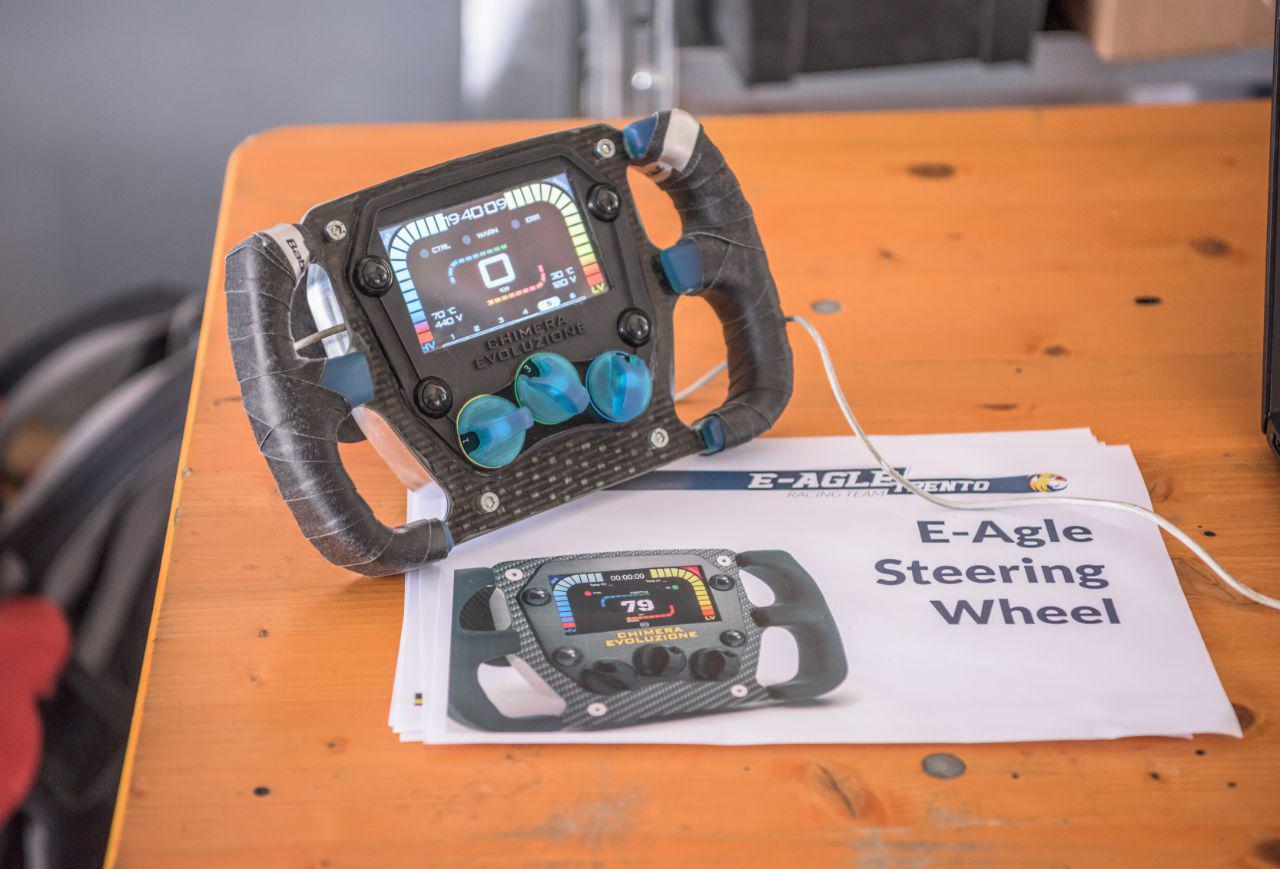
\includegraphics[width=0.75\textwidth]{./figures/steeringwheelPresentation.jpg}
    \caption{Presentazione del Volante - Varano Luglio 2018}
\end{figure}

Nel Luglio 2018, durante la partecipazione alla tappa italiana del campionato presso il circuito di Varano (PR), ho avuto la prima conferma da parte 
di esterni sulla qualità del nostro lavoro, delle scelte tecniche e di sviluppo che sono state fatte durante l'anno.
La riconferma di ciò è stata la premiazione da parte di Alessandro Pocecco, Project Leader della parte Elettronica di Lamborghini, 
con il premio per \emph{Best HMI Solution}.
La soluzione che abbiamo deciso di presentare è stata valutata non solo come prodotto, ma soprattutto per la presentazione che ho avuto
l'onore di condurre, mostrando in particolare il nostro approccio durante la fase di design del prodotto e le metodologia di sviluppo.
Il giudice si è complimentato per l'impegno, dandoci numerosi consigli e facendo apprezzamenti sulle scelte tecniche in base ai nostri requisiti,
che sono state motivate utilizzando un approccio molto più vicino al mondo lavorativo che a quello didattico.

Ad Agosto 2018, durante la tappa di Barcellona, ci è stato fatto presente della mancanza di una vera soluzione telemetrica, questo perchè il Volante
è stato pensato per essere utilizzato principalemente dal Pilota e per i test, ma non per la raccolta dati. 
Da qui è nata la necessità di sviluppare una appliciazione a microservizi basata sulla comunicazione wireless della macchina 
con un dispositvo esterno per raccoglierne i dati e visualizzarli in real-time con il salvataggio in database per poter poi fare delle analisi più
precise sulla nostra monoposto.

\section{Sviluppi Futuri}

Per quanto riguarda il Volante, grazie ai feedback dei giudici, delle persone che ci hanno lavorato come utenti e da chi l'ha sviluppato abbiamo raccolto
molte informazioni sul come poterlo migliorare.
Per poter avere un'analisi più precisa sulle risosrse da impiegare al miglioramente del dispositivo
abbiamo deciso di utilizzare un'approccio qualitativo diverso.
L'approccio consiste nel definire parametri misurabili in fase di progettazione, molto simile a quello utilizzato dal gruppo telemetria 
ma senza l'utilizzo di variabili.
Questa tecnica viene chiamata \textbf{QFD} e consiste nel tenere conto delle necessità del cliente esterno 
per poter venire il più possibile incontro a quelle del cliente interno (sviluppatori e designer).
È importante precisare che il nostro principale competitor siamo noi stessi, con la soluzione che abbiamo 
implementato nel 2018.
Al momento non sono presenti all'interno della competizione di Formula SAE prodotti custom simili al nostro,
curati sia dal punto di vista grafico che funzionale, ma soluzioni per il motor-sport in generale acquistate e utilizzate dalle squadre.

\begin{figure}[hbt!]
    \centering
    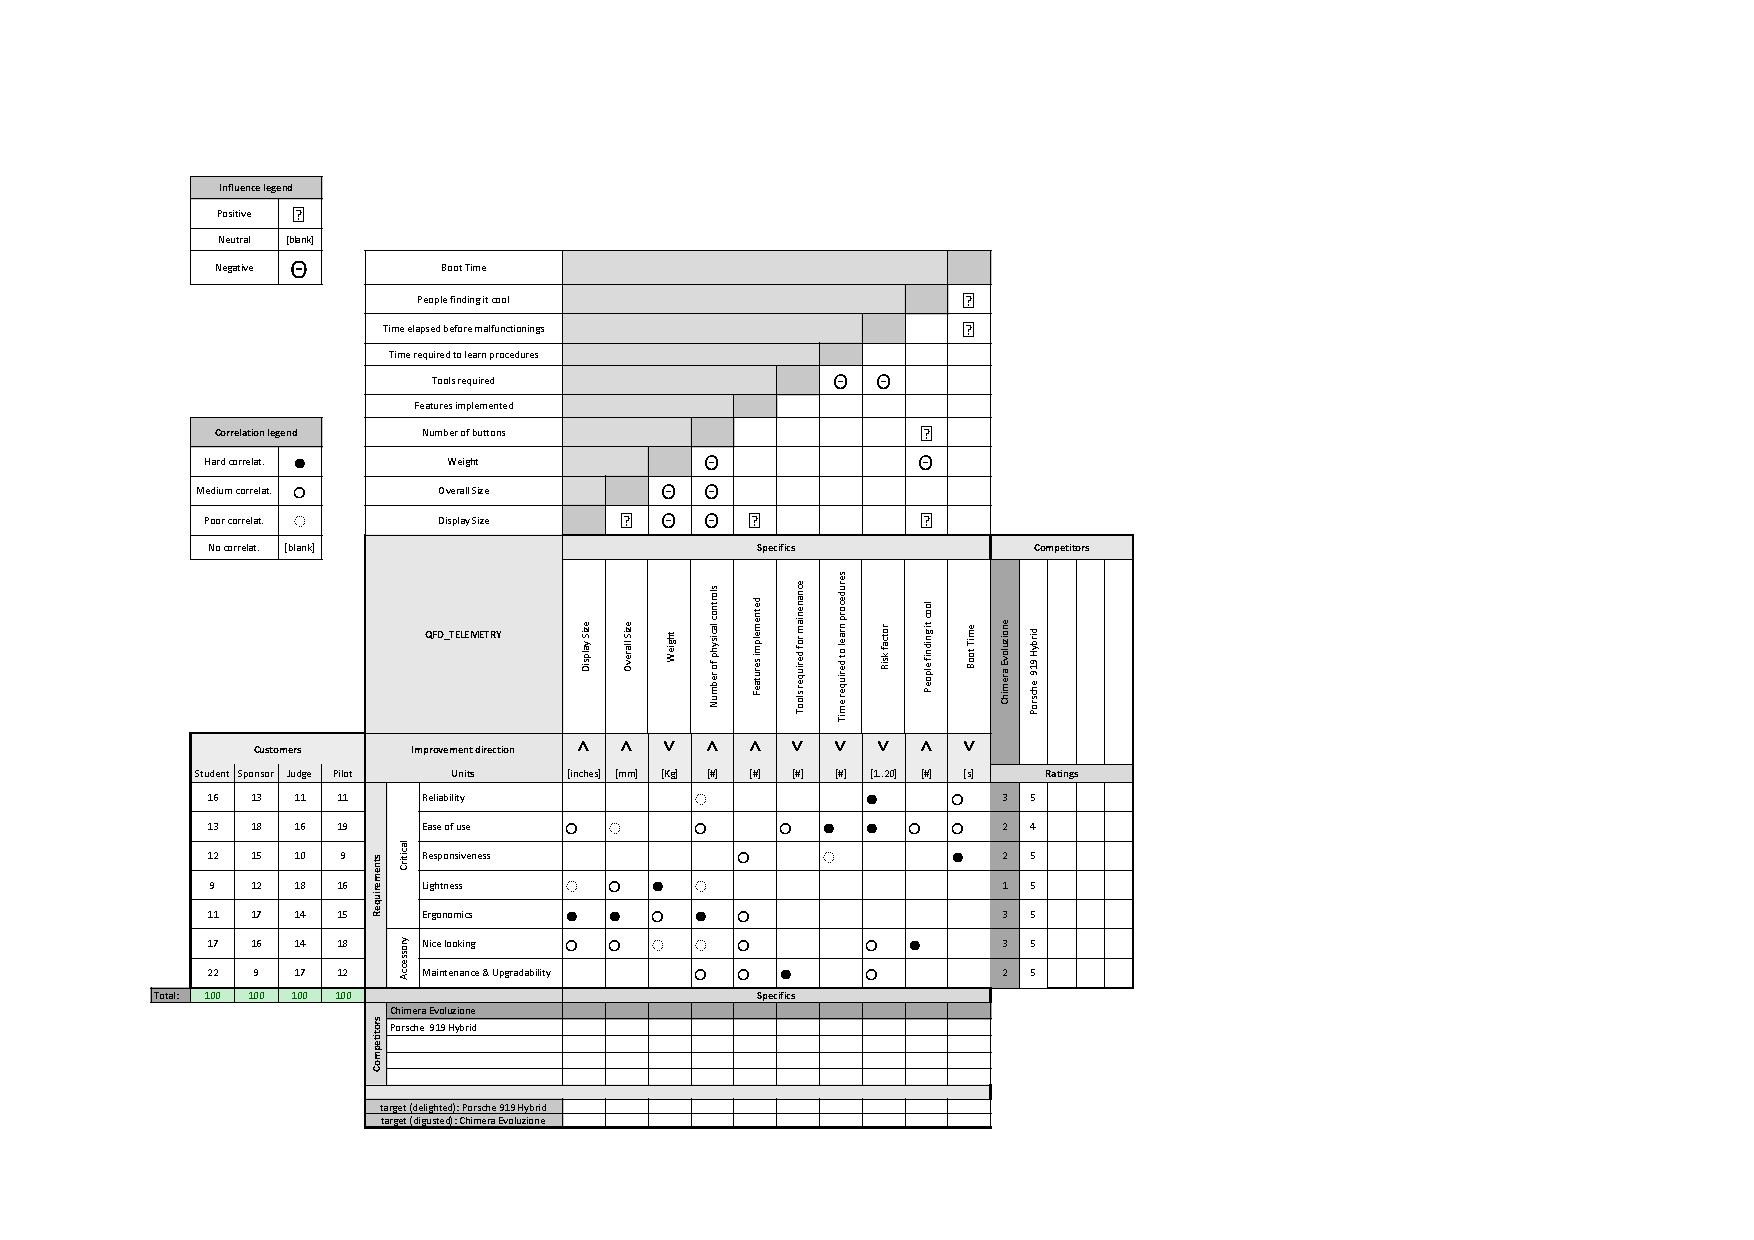
\includegraphics[width=0.95\textwidth]{./figures/QFD_Telemetry.pdf}
    \caption{QFD Ottobre 2018}
\end{figure}

Dalla QFD sono emersi diversi punti importanti su cui lavorare, qui schematizzati:

\begin{itemize}
    \item Case ridisegnato per renderlo facilemente aggiornabile grazie al ausilio di una 
            mascherina che può essere rimossa per poter lasciare il case uguale e ridurre i costi.
    \item Impugnatura ergonomica su misura ottenuta attraverso scanner 3D. 
    \item Cambiare hardware, scelta di una scheda più potente e ridurre lo spazio della componentistica hardware, 
        la soluzione di riferimento è un Raspberry Pi CM3 con memoria SD.
    \item Gestire su due Thread il programma, uno per la lettura del Can-Bus l'altro per l'interfaccia.
    \item Migliorare i tempi di boot del sistema operativo. Grazie al premio vinto 
        abbiamo potuto conttattare \emph{Qt} per una sponsorizzazione e ora abbiamo a disposizione 
        l'intera suite per lo sviluppo emebedded che, attraverso anche alla collaborazione dei loro
        partner, ci permetterà di utilizzare al massimo le potenzialità del loro framework.
    \item Aggiornare l'interfaccia proponendo più versioni in base al caso d'uso e il pilota.
    \item Inserire led di notifica sopra al display, questa funzionalità è ancora da definire ma una 
        sua prima applicazione può essere notificare certe informazioni al pilota o a 
        chi fa i test e in fase di gara vedere il bloccaggio delle ruote. 
    \item Aggiornare i dispositivi di input, inserendo altri due paddlee un bottone, uno per il launch control e 
        l'altro da utilizzare come marker (ripristinando la soluzione della comunicazione radio).
    \item Aumentare la dimensione del display da 4.3" a 5", per poter integrare nuove funzionalità e avere un display qualitativamente migliore.
    \item Rendere ancora più intuitiva l'interfaccia grazie a tasti con scritte colorate e automatizzare 
        alcune procedure alle quali il pilota non interessa conoscere attraverso un bottone di "start automatico", mantenendo e migliorando la veccia procedura.
    \item Aggiungere la possibilità di premere più tasti contemporaneamente per attivare altre funzioni.
    \item Migliroare il feedback per il pilota, attraverso il flash di colori e informazioni, 
        così da poter essere informati più velocemente sullo stato della macchina. 
\end{itemize}

\begin{figure}[h!]
    \centering
    \begin{minipage}{0.5\textwidth}
        \centering
        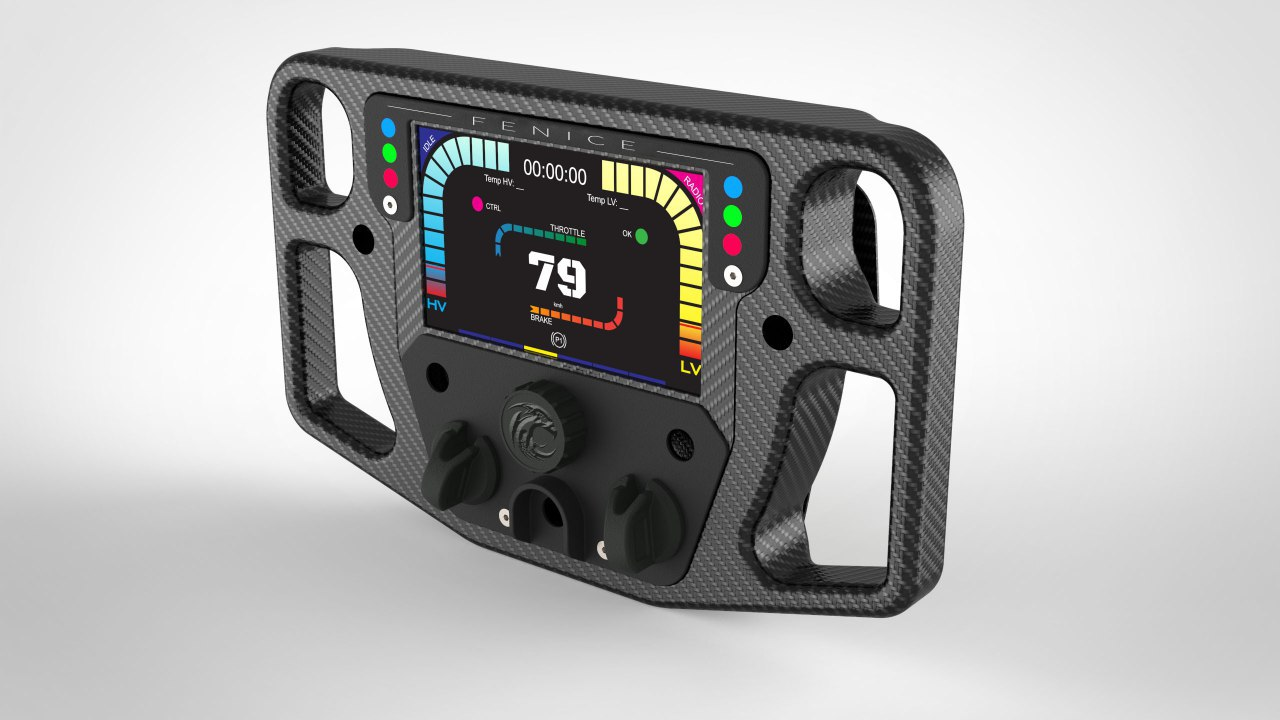
\includegraphics[width=0.9\textwidth]{./figures/volanteFenice.jpg}
    \end{minipage}\hfill
    \begin{minipage}{0.5\textwidth}
        \centering
        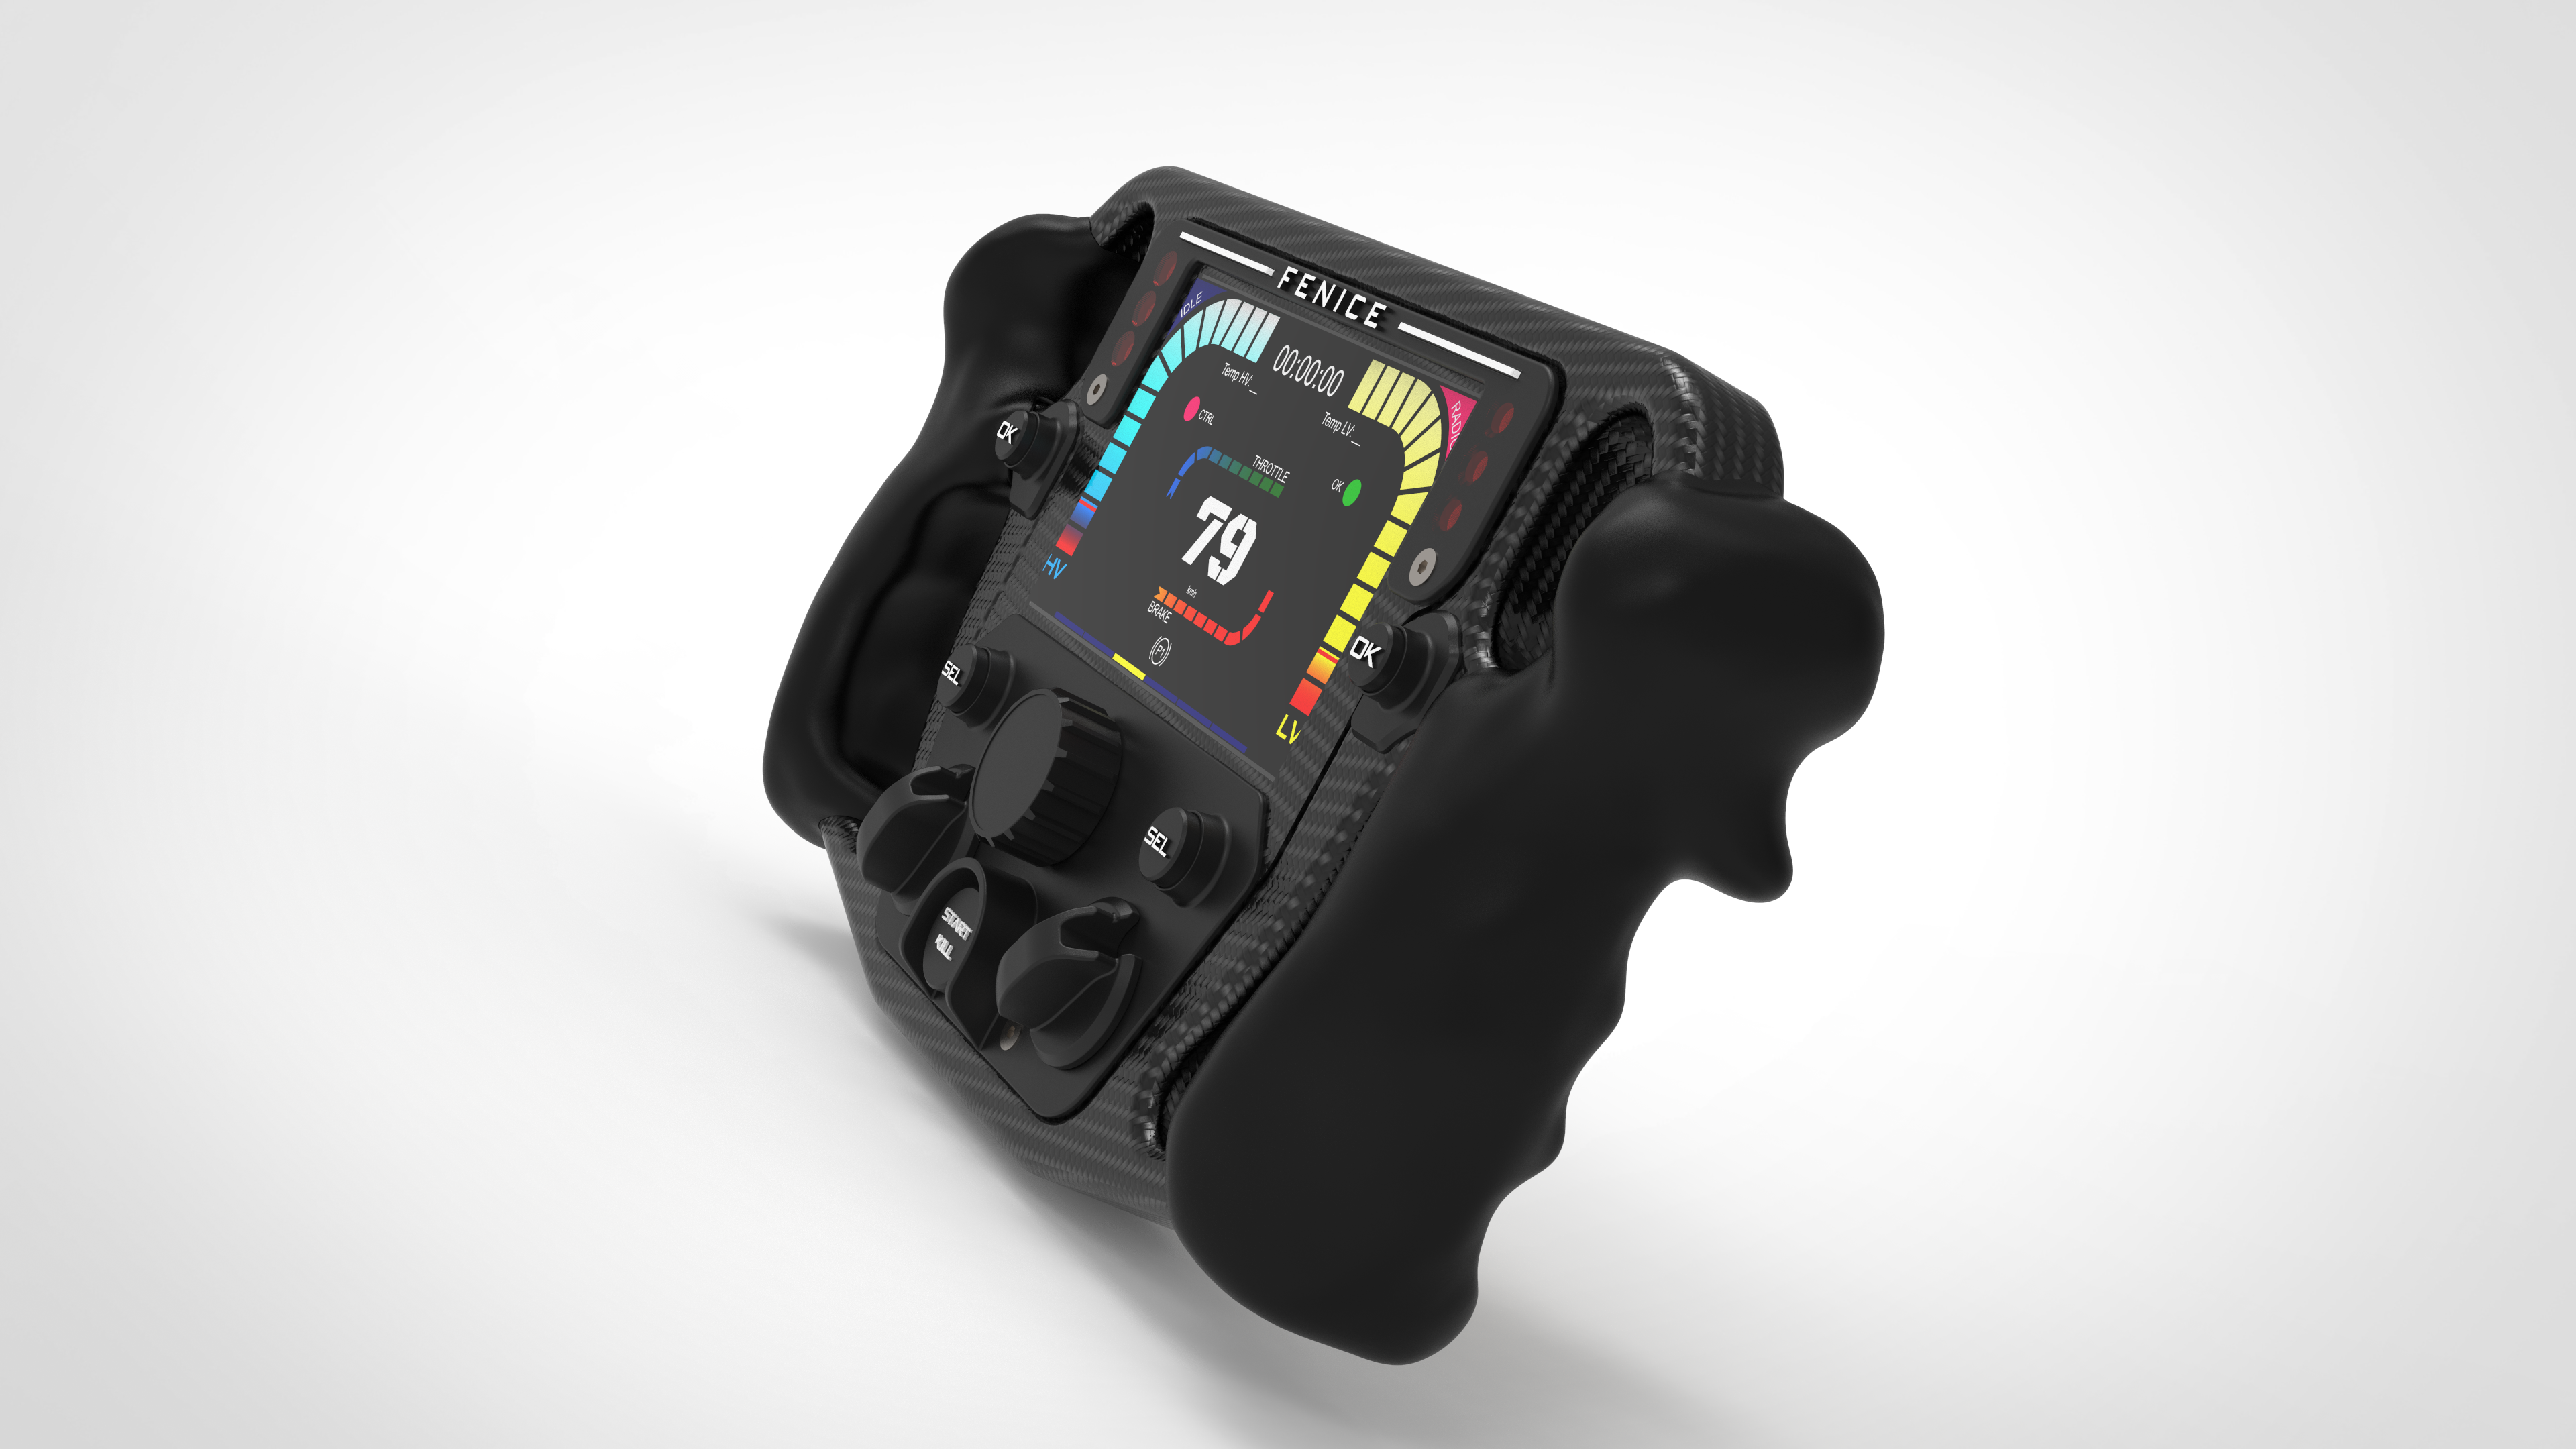
\includegraphics[width=0.9\textwidth]{./figures/volanteFenice1.png}
    \end{minipage}
    \caption{Primo Mockup del Volante di Fenice}
\end{figure}

% \begin{figure}[hbt!]
%     \centering
%     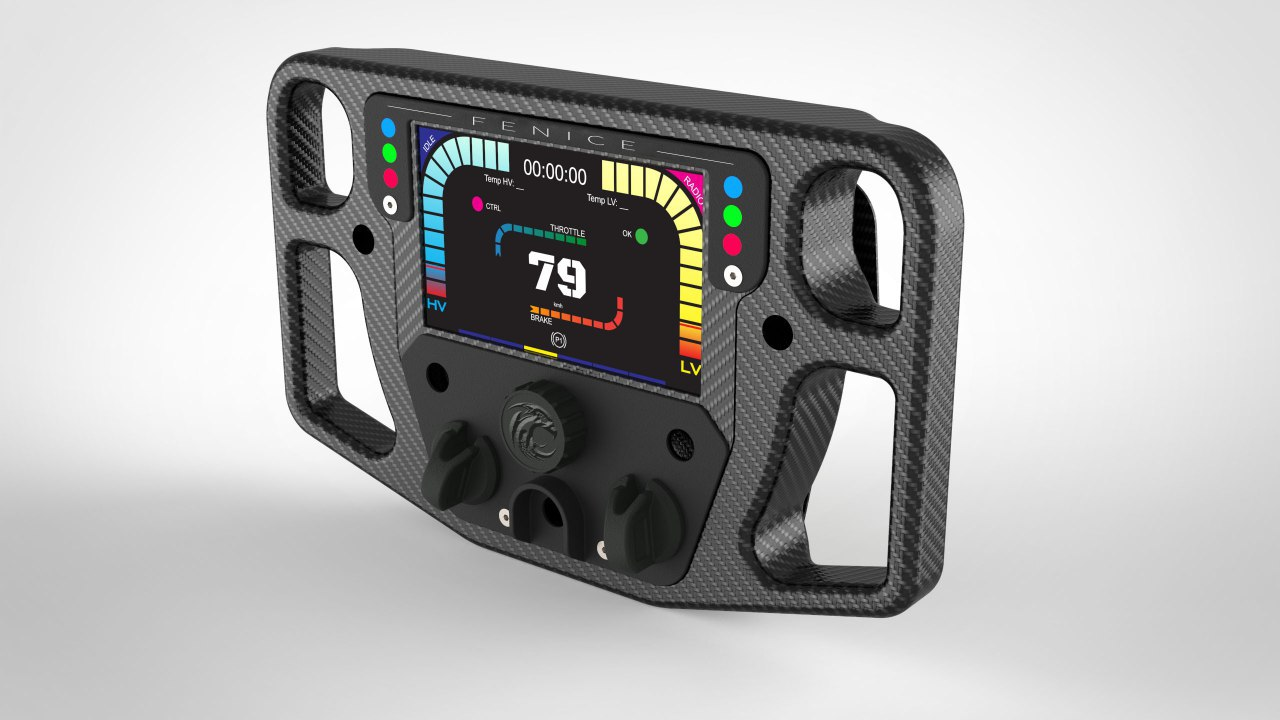
\includegraphics[width=0.75\textwidth]{./figures/volanteFenice.jpg}
%     \caption{Primo Mockup del Volante Fenice}
% \end{figure}

% \begin{figure}[hbt!]
%     \centering
%     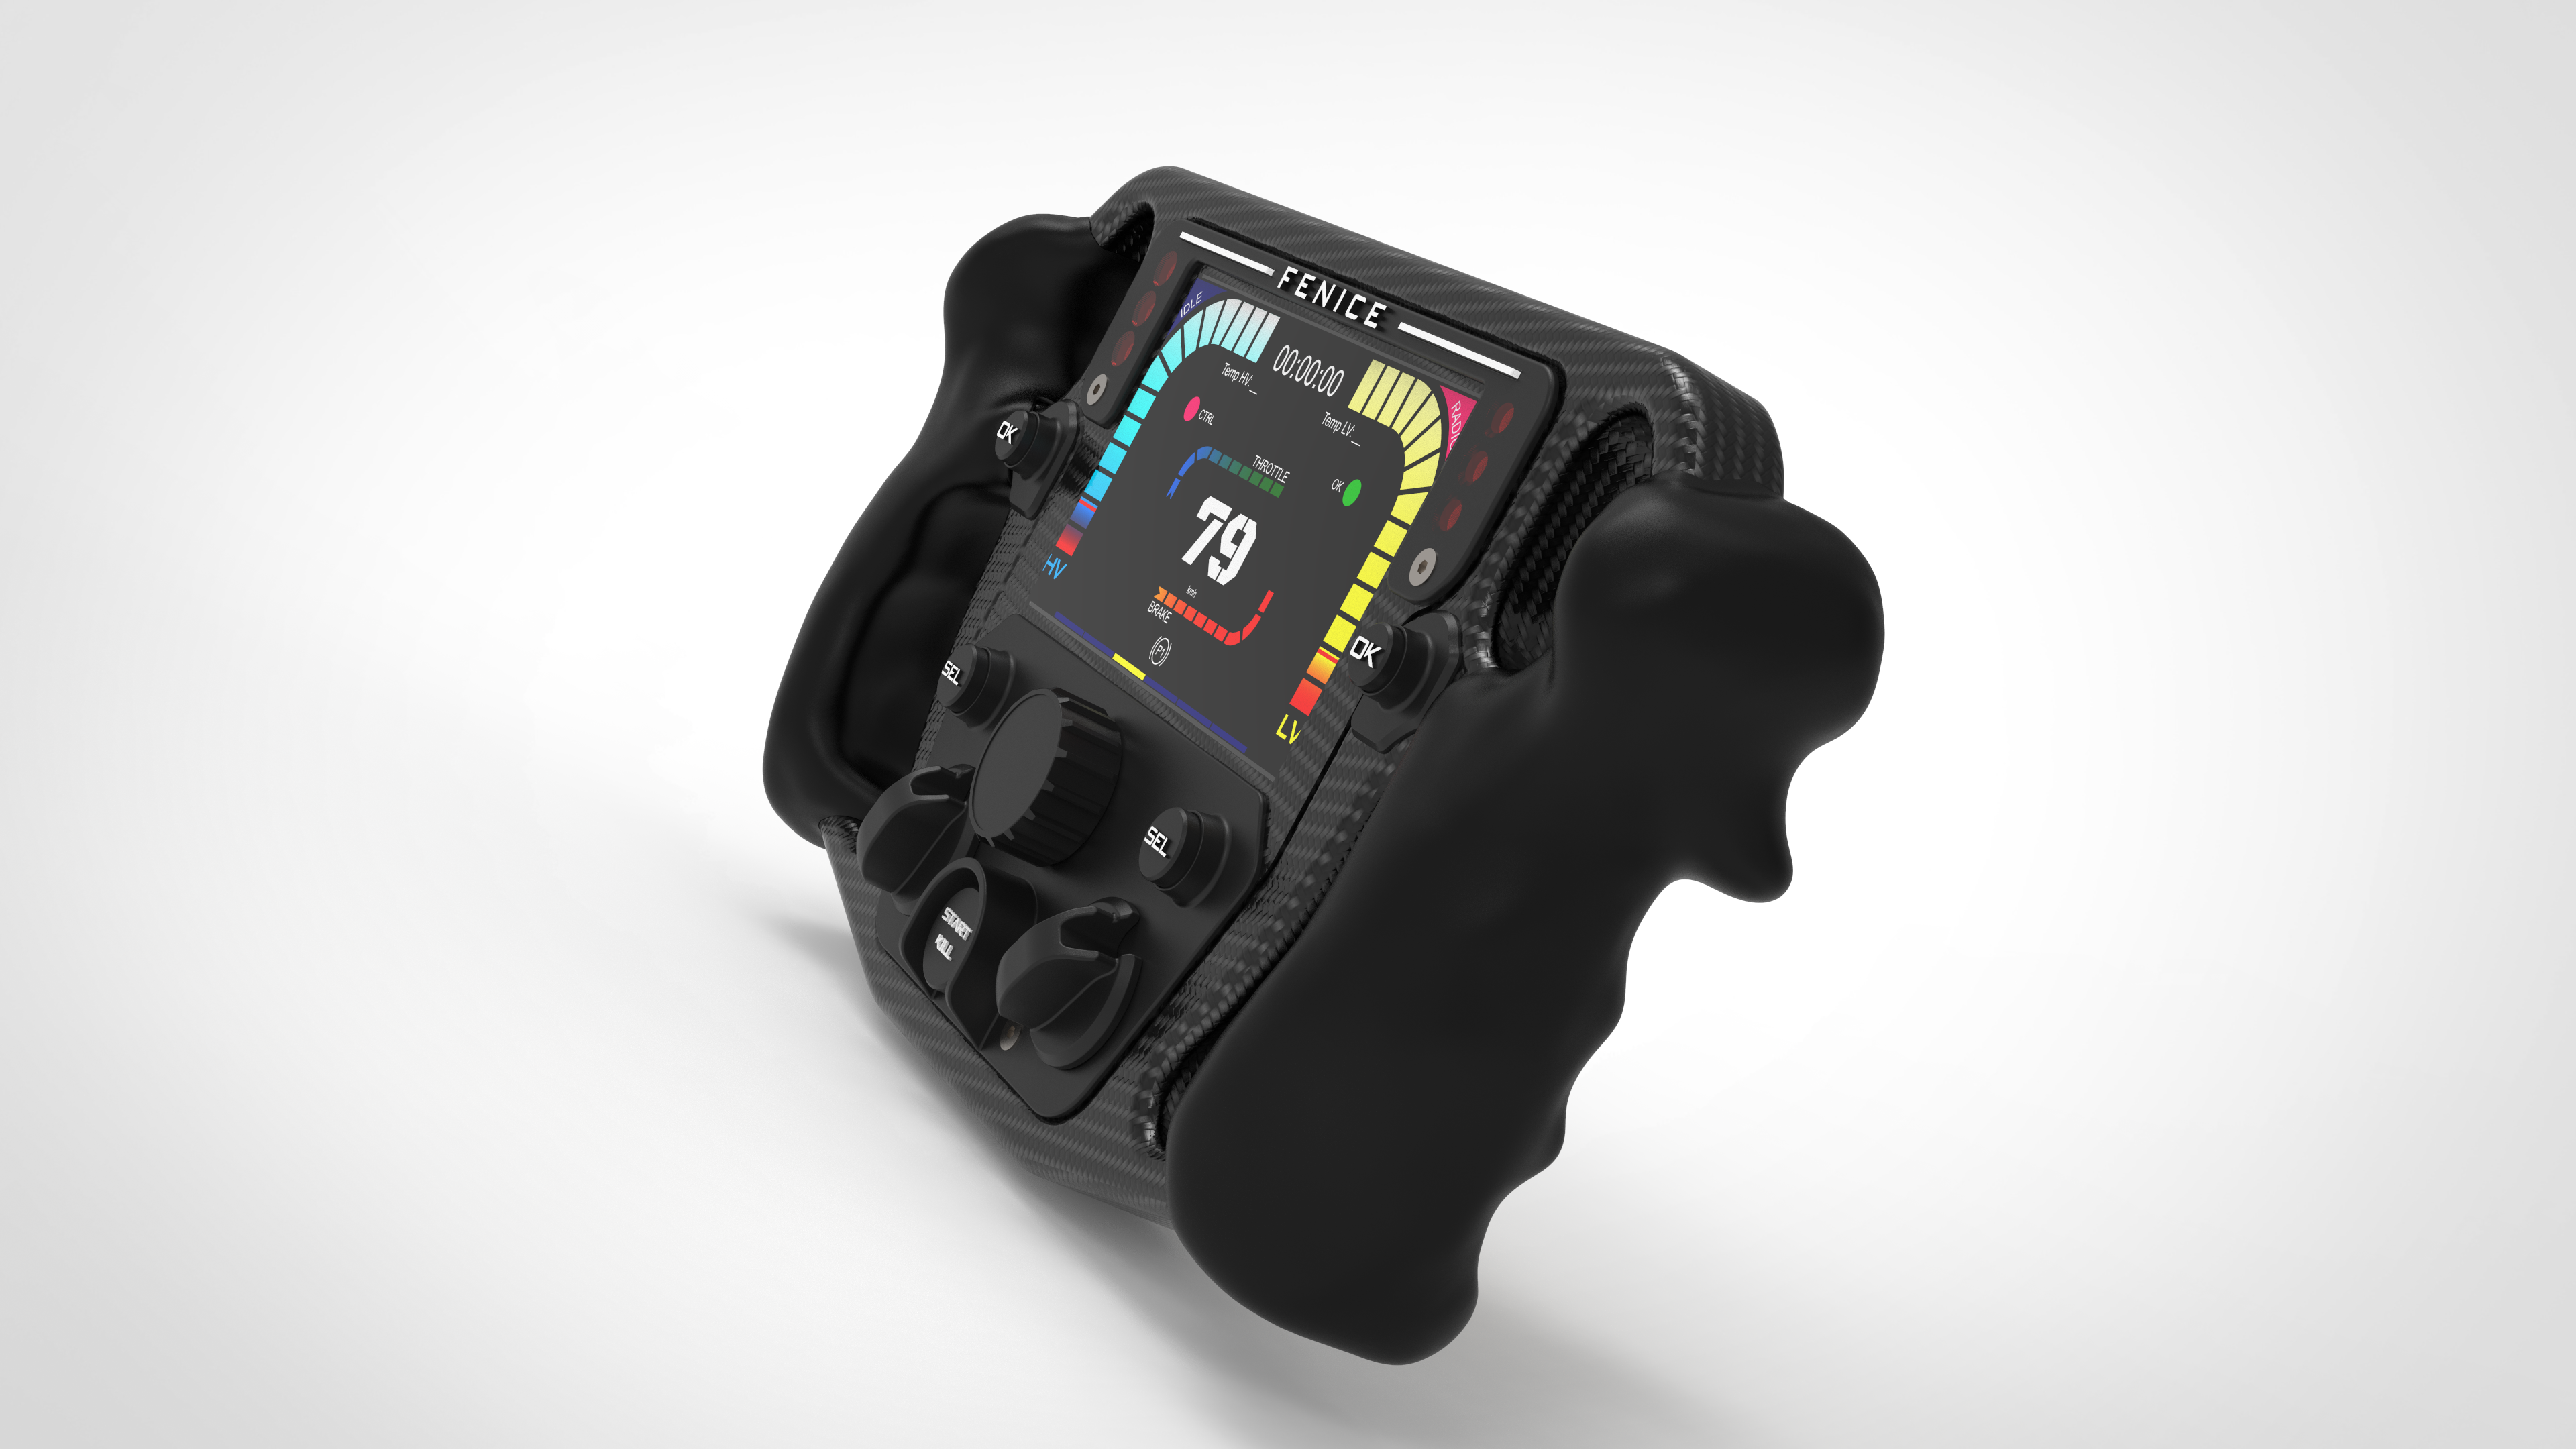
\includegraphics[width=0.75\textwidth]{./figures/volanteFenice1.png}
%     \caption{Impugnatura Ergonomica Scannerizzata 3D}
% \end{figure}

Il progetto del Volante non è da intedersi come finito, ma come continua ricerca di soluzioni migliori.
Il test su altri dispositvi e con altre tecnologie mostra la facilità/difficoltà di integrarsi al nostro progetto, 
la scelta di effettuare questo tipo di prove viene preso dal singolo valutando la fattibilità e l'interesse personale.
Un esempio è il framework che utilizza il gruppo Volkswagen, in particolare Audi con il loro premiato MMI. È sicuramente un ottima soluzione, ma le considerazioni fatte sui prezzi delle licenze,
il taget dei loro clienti (principalmente designer) ci ha spinto scartarlo optando per soluzioni open-source, poco costose e che sfruttano tecnologie che possono mostrarsi polifunzionali. 

\newpage

% \textbf{TODO del futuro}

% Attraverso queste funzionalità e design siamo riusciti ad avere: 
% \begin{itemize}
%     \item Toold Debug (canutils, candump, le tab)
%     \item Tool + stabile al momento in macchina (non si rompe in quanto è in lettura e mostra lo stato della macchina sempre)
% \end{itemize}

% mettere feedback del display per procedure
% ripensare alle procedure migliorando l'efficenza e limitare l'aggiornamento della grafica i 30fps 
% mettere su due thread la ui il backend

% problemi e come li risolviamo (fenice hw, so miglioratoe, nuove interfaccia 5", tasti colorati, notifica pressione tasti nuove funzionalità della telemetria) 
% approcio nuovo grazie alla sponsorizzazione di qt, valutazione anche di framework alternativi, vedi kanzi usata dal gruppo audi, ma più orientato ad un approccio 
% da desginer che da studenti di ingegeria, oltre a questo risulta essere costoso e "innarivabile" per il nostro progetto (volante) che si fonda sullo spendere
% il meno possibile e realizzare le migliori soluzioni dando il più possibile del nostro

    \chapter{Conclusioni}

% esperienza complessiva
% cosa ho fato e cosa ho imparato
% a cosa mi è servito e cosa ho intenzione di fare

L'esperienza all'interno del team mi ha permesso di applicare le conoscenze informatiche
e maturarne altre in settori che non avrei mai potuto conoscere se non grazie ad un progetto del genere.
I sistemi embedded e il design dei prodotti mi è sempre piaciuto ed avere la possibilità di lavorarci è stato
motivo di grande soddisfazione oltre che avermi permesso di individuare i possibili sviluppi di un percorso professionale futuro.
Lavorare sul volante e collaborare con altre persone, professori e studenti, mi ha aiutato a fare 
mie metodologie di sviluppo e le tecnologie utilizzate.
Da Settembre 2018 mi sono occupato personalmente della parte software del Volante, grazie alle conoscenze maturate
nel campo dei sistemi operativi e dello sviluppo con Qt, 
lasciando la parte elettronica e meccanica a Daniele Faccinelli e Ciro Malacarne.
L'esperienza complessiva mi ha permesso di entrare in contatto con persone altamente specializzate nel settore dell'automotive, 
che riconoscono i nostri sacrifici e il lavoro che c'è dietro ad un progetto di questo tipo. 
Reputo il progetto molto impegnativo, ma grazie all'avanzamento dei lavori del Volante e l'entusiasmo 
della squadra e dei collaboratori, ho intenzione di continuare l'esperienza nel team per terminare il progetto telemetria
e lo sviluppo del Volante.
    
  \endgroup

  % bibliografia in formato bibtex
  %
  % aggiunta del capitolo nell'indice
  \addcontentsline{toc}{chapter}{Bibliografia}
  % stile con ordinamento alfabetico in funzione degli autori
  \bibliographystyle{plain}
  \bibliography{biblio}

  \titleformat{\chapter}
      {\normalfont\Huge\bfseries}{Allegato \thechapter}{1em}{}

\end{document}
